\chapter{三角函数的性质与图象}

在展开本章具体内容之前,首先应明确两点:(1)研究函数性质的依据是函数的定义。对于三角函数来讲,它的每种函数的定义与其相应的三角函数线的定义是彼此等价的(一种是代数形式,一种是几何形式、代数形式便于计算,几何形式形象直观). 因此,研究中根据需要我们可以灵活地选用任何一种形式;(2)在中学阶段,研究\textbf{函数的初等性质}主要限于以下五个方面:
\begin{enumerate}
    \item 定义域(我们用$D$表示它);
    \item 值域(对$D$而言,是整体性质);
    \item 增减性(对$D$的某个子区间而言,是局部性质),
    \item 奇偶性(对$D$而言,是整体性质);
    \item 周期性(对$D$而言,是整体性质)。
\end{enumerate}

在1.4节,我们曾经利用单位圆,对三角函数的某些性质(定义域、值域、五组诱导公式)做过初步的探究。本章将在此基础上完成对三角函数初等性质的全面研究,并画出各种三角函数的图象。

\section{关于三角函数定义域与值域的补充}

{练习}:
 根据三角函数(或三角函数线)的定义填表:
\begin{center}
\begin{tabular}{c|c|c|c|c|c|c}
\hline
函数 & $\sin\alpha=y$&$\cos\alpha=x$& $\tan\alpha=\frac{y}{x}$&$\cot\alpha=\frac{x}{y}$&$\sec\alpha=\frac{1}{x}$&$\csc\alpha=\frac{1}{y}$\\
\hline
定义域&&&&&\\
\hline
值域&&&&&\\
\hline
\end{tabular}
\end{center}    

\begin{example}
    求下列函数的定义域。
\begin{multicols}{2}
\begin{enumerate}[(1)]
    \item $f(\alpha)=\sqrt{\cot\alpha\cdot\csc\alpha}$
    \item $f( \beta ) = \sqrt {\sin \beta }+\lg(2\cos\beta+1)$
    \item $f( x) = \frac {\sin x\cdot \tan \left ( x- \frac \pi 4\right ) }{2\cos x- 1}$
\end{enumerate}    
\end{multicols}

\end{example}

\begin{solution}
\begin{enumerate}[(1)]
    \item 要 使 $f( \alpha )$ 有意义,须$\cot \alpha\cdot\csc\alpha\ge 0$, 即$\cot\alpha$与$\csc\alpha$同号或积为零。在图 3.1 中我们分别标出这两个函数值的符号。“可见动点应落在实线画出的弧上(注意:点$B$、$C$在
内,点$A$除外),

$\therefore\quad \alpha\in\left(0+2k\pi,\; \frac{\pi}{2}+2k\pi\right]\cup\left[\frac{3\pi}{2}+2k\pi,\; 2\pi+2k\pi\right),\quad k\in\Z$

\noindent
\begin{minipage}{.45\textwidth}
\centering
\begin{tikzpicture}[>=stealth]
\draw[->](-2.5,0)--(2.5,0)node[below]{$x$};
\draw[->](0,-2.5)--(0,2.5)node[left]{$y$};
\draw(0,-1.5) arc (-90:90:1.5);
\draw[dashed](0,1.5) arc (90:270:1.5);
\foreach \x in {1.5, -1.5}
{
    \draw[fill=white] (\x,0)circle(1.5pt);
    \draw[fill] (0,\x)circle(1.5pt);
}
\node at (1.5,0)[above right]{$A$};
\node at (0,1.5)[above right]{$C$};
\node at (0,-1.5)[below right]{$B$};
\node [below left]{$O$};
\node at (.5,.75)[text width=1cm, align=center]{$+$\\$+$};
\node at (-.5,.75)[text width=1cm, align=center]{$-$\\$+$};
\node at (.5,-.75)[text width=1cm, align=center]{$-$\\$-$};
\node at (-.5,-.75)[text width=1cm, align=center]{$+$\\$-$};

\end{tikzpicture}   
\captionof{figure}{} 
\end{minipage}\hfill
\begin{minipage}{.45\textwidth}
\centering
\begin{tikzpicture}[>=stealth]
\draw[->](-2.5,0)--(2.5,0)node[below]{$x$};
\draw[->](0,-2.5)--(0,2.5)node[left]{$y$};
\draw(0,0)node[below right]{$O$}circle (1.5);
\draw[dashed](-0.75,-2.5)--(-0.75,2.5);
\draw[thick](120:1.5)--(0,0)--(-120:1.5);
\draw[fill=white] (120:1.5)node[above left]{$P$}  circle(1.5pt);
\draw[fill=white] (-120:1.5)node[below left]{$Q$}  circle(1.5pt);
\draw[->, thick](0,0)--(-.75,0)node[below left]{$N$};
\node at (1.5,0)[below right]{$A$};
\draw[->](.35,0) arc (0:120:.35);
\node at (60:.6){$\tfrac{2\pi}{3}$};

\end{tikzpicture}    
\captionof{figure}{} 

\end{minipage}


\item 要使$f(\beta)$有意义,须
\begin{align}
    \sin\beta\ge 0 \tag{1}\\
    2\cos\beta +1>0\Longleftrightarrow \cos\beta>-\frac{1}{2}\tag{2}
\end{align}
在单位圆上(图3.2)画出余弦线$\VEC{ON}=-\frac{1}{2}$,过$N$作$PQ\parallel y$轴,则满足(2)的动点应落在$\widearc{QAP}$上,满足(1)的动点应落在$x$轴(含$x$轴)上方的弧上. 从而,满足 不等式(1)(2)的动点应落在$\widearc{AP}$上.

$\therefore\quad \beta\in \left[0+2k\pi,\; \frac{2\pi}{3}+2k\pi\right),\quad k\in\Z$

\item 要使$f(x)$有意义,须
\[\begin{cases}
    x-\frac{\pi}{4}\ne\frac{\pi}{2}+k\pi\Longleftrightarrow x\ne \frac{3\pi}{4}+k\pi\quad (k\in\Z)\\
    \cos x\ne \frac{1}{2}
\end{cases}\]
在单位圆上,满足不等式组的$x$的对应点应落在图3.3中实线画出的弧上,即$x\in\R$,且$x\ne \frac{3\pi}{4}+k\pi$,$x\ne \frac{\pi}{3}+2k\pi$,$x\ne \frac{5\pi}{3}+2k\pi\; (k\in\Z)$,或者表示成
\[\begin{split}
x\in &\left(\frac{\pi}{3}+2k\pi,\; \frac{3\pi}{4}+2k\pi\right)\cup \left(\frac{3\pi}{4}+2k\pi,\; \frac{5\pi}{3}+2k\pi\right)\\
&\cup \left(\frac{5\pi}{3}+2k\pi,\; \frac{7\pi}{4}+2k\pi\right)\cup \left(-\frac{\pi}{4}+2k\pi,\; \frac{\pi}{3}+2k\pi\right),\quad k\in\Z
\end{split}\]

\noindent
\begin{minipage}{.45\textwidth}
    \centering
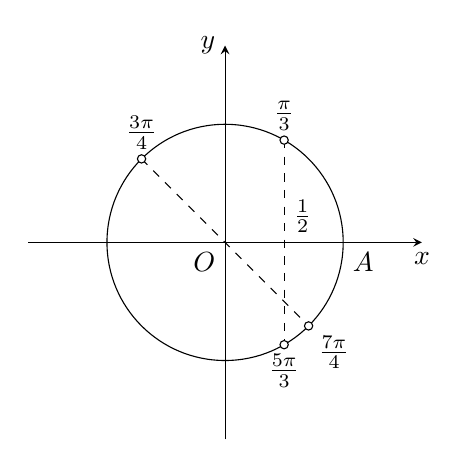
\begin{tikzpicture}[>=stealth]
    \draw[->](-2.5,0)--(2.5,0)node[below]{$x$};
    \draw[->](0,-2.5)--(0,2.5)node[left]{$y$};
    \draw(0,0)node[below left]{$O$}circle (1.5);
    \draw[dashed] (60:1.5)node[above]{$\frac{\pi}{3}$}--(-60:1.5)node[below]{$\frac{5\pi}{3}$};
    \draw[dashed] (135:1.5)node[above]{$\frac{3\pi}{4}$}--(-45:1.5)node[below right]{$\frac{7\pi}{4}$};
\foreach \x in {60,-60,135,-45}
{
    \draw[fill=white](\x:1.5) circle(1.5pt);
}
\node at (.75,0)[above right]{$\frac{1}{2}$};
\node at (1.5,0)[below right]{$A$};
\end{tikzpicture}
    \captionof{figure}{}
\end{minipage}
\hfill
\begin{minipage}{.45\textwidth}
    \centering
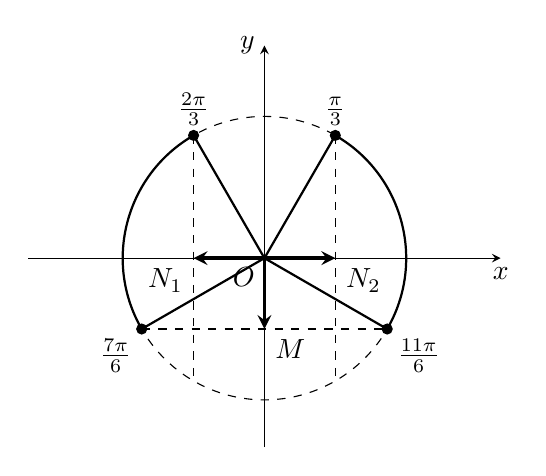
\begin{tikzpicture}[>=stealth, scale=1.2]
    \draw[->](-2.5,0)--(2.5,0)node[below]{$x$};
    \draw[->](0,-2)--(0,2.25)node[left]{$y$};
    \draw[dashed](0,0)node[below left]{$O$}circle (1.5);
    \draw[dashed] (60:1.5)node[above]{$\frac{\pi}{3}$}--(-60:1.5);
    \draw[dashed] (120:1.5)node[above]{$\frac{2\pi}{3}$}--(-120:1.5);
\foreach \x in {60,-30,120,-150}
{
    \draw[fill](\x:1.5) circle(1.5pt);
    \draw[thick](\x:1.5)--(0,0);
}
\draw[thick](-30:1.5)node[below right]{$\frac{11\pi}{6}$} arc (-30:60:1.5);
\draw[thick](210:1.5)node[below left]{$\frac{7\pi}{6}$} arc (210:120:1.5);
\draw[dashed](210:1.5)--(-30:1.5);
\draw[very thick,->](0,0)--(0,-.75)node[below right]{$M$};
\draw[very thick,->](0,0)--(-.75,0)node[below left]{$N_1$};
\draw[very thick,->](0,0)--(.75,0)node[below right]{$N_2$};
\end{tikzpicture}
\captionof{figure}{}
\end{minipage}


\end{enumerate}
\end{solution}

\begin{example}
    解不等式组:
\begin{align}
    \sin x>-\frac{1}{2} \tag{1}\\
    |\cos x|\ge \frac{1}{2}\tag{2}
\end{align}
\end{example}

\begin{solution}
在单位圆上分别作出正弦线$\VEC{OM}=-\frac{1}{2}$,余弦线$\VEC{ON_1}=-\frac{1}{2}$,$\VEC{ON_2}=\frac{1}{2}$,过点$M$、$N_1$、$N_2$分别作$x$轴和$y$轴的平行线(图3.4)。可知满足不等式组的动点应落在实线画出的弧上,从而有
\[x\in\left[\frac{2\pi}{3}+2k\pi,\; \frac{7\pi}{6}+2k\pi\right)\cup \left(-\frac{\pi}{6}+2k\pi,\; \frac{\pi}{3}+2k\pi\right],\quad k\in\Z\]

\end{solution}

\begin{thm}{思考题}
    上式中后一个区间写成下面的形式,错在哪里?
\[\left(\frac{11\pi}{6}+2k\pi,\; \frac{\pi}{3}+2k\pi\right),\quad k\in\Z\]
\end{thm}

\begin{example}
   写出使下列不等式成立的$x$的集合: 
\begin{multicols}{2}
\begin{enumerate}[(1)]
    \item  $\sqrt{3}+\tan x\leq 0$
    \item $\cot x-2\geqslant 0$ 
\end{enumerate}
\end{multicols}
\end{example}

\begin{solution}
\begin{enumerate}[(1)]
    \item 由原式,得$\tan x\leqslant-\sqrt{3}$,

$\therefore\quad x\in \left ( \frac \pi 2+ k\pi , \frac {2\pi }3+ k\pi \right ],\; k\in \Z$(图3.5).

\noindent
\begin{minipage}{.45\textwidth}
\begin{tikzpicture}[>=stealth]
\draw[->](-2.5,0)--(2.5,0)node[below]{$x$};
\draw[->](0,-2.5)--(0,2.5)node[left]{$y$};
\node [below left]{$O$};
\node at (1.5,0)[below right]{$A$};
\draw[dashed](0,0) circle(1.5);
\draw(1.5,0)--(1.5,-1.5*1.732)node[below]{$\sqrt{3}$};
\draw[dashed](120:1.5)node[above left]{$\frac{2\pi}{3}$}--(1.5,-1.5*1.732);
\draw[very thick](0,1.5) arc (90:120:1.5);
\draw[very thick](0,-1.5) arc (-90:-60:1.5)node[below]{$\frac{5\pi}{3}$};
\draw[fill=white](0,-1.5)circle(1.5pt);
\draw[fill=white](0,1.5)circle(1.5pt);
\draw[fill](120:1.5)circle(1.5pt);
\draw[fill](-60:1.5)circle(1.5pt);
\end{tikzpicture}    
\captionof{figure}{}
\end{minipage}\hfill
\begin{minipage}{.45\textwidth}
\begin{tikzpicture}[>=stealth]
\draw[->](-2.5,0)--(2.5,0)node[below]{$x$};
\draw[->](0,-2.5)--(0,2.5)node[left]{$y$};
\node [below right]{$O$};
\node at (1.5,0)[below right]{$A$};
\draw[dashed](0,0) circle(1.5);
\draw(0,1.5)--(3,1.5)node[right]{2};
\draw[dashed](-180+26.56:1.5)node[below left]{$\pi+x'$}--(3,1.5);
\draw[very thick](1.5,0) arc (0:26.56:1.5)node[right]{$x'$};
\draw[very thick](-1.5,0) arc (180:206.56:1.5);
\draw[fill=white](-1.5,0)circle(1.5pt);
\draw[fill=white](1.5,0)circle(1.5pt);
\draw[fill](26.56:1.5)circle(1.5pt);
\draw[fill](-180+26.56:1.5)circle(1.5pt);

\end{tikzpicture}    
\captionof{figure}{}
\end{minipage}

\item 由原式,得
$\cot x\ge 2$,对于$x$的边界值$x'$来说,$\cot x'=2$不是特殊角,我们可以用量角器量出$x'$的值(在精度要求不高的情况下,这样做是可行的),从而
$x\in (0+k\pi,\; x'+k\pi],\quad k\in\Z$(图3.6)。
\end{enumerate}
\end{solution}

\begin{remark}
求三角函数式的定义域,归结为解三角不等式(或不等式组)。可以先在周内角范围内运用三角函数线进行研究,然后再考虑一般情况。
\end{remark}

\begin{thm}
    {思考题} 你能说出下列三角函数的值域吗?
\begin{multicols}{3}
\begin{enumerate}[(1)]
    \item $y=\sin x+3$
    \item $y=2\cos x$
    \item $y=-3\sin x+1$
\end{enumerate}    
\end{multicols}
\end{thm}

\begin{example}
试求函数$f(x)=\sin x+\cos x$的值域。
\end{example}

\begin{thm}
  {问1}由$-1\le \sin x\le 1$, $-1\le \cos x\le 1$, $f(x)$的值域是否为$[-2,2]$呢?
\end{thm}

\begin{analyze}
$f(x)$的值域不是$[-2,2]$。这是因为当$\sin x$取得最小值$-1$时,$x=-\frac{\pi}{2}+2k\pi,\; (k\in\Z)$,此时$\cos x$并不能取得最小值$-1$.对于$\sin x$取最大值的情况也是类似的。因此,欲求$f(x)$的值域,应先化简$f(x)$.
\end{analyze}

\begin{solution}
    根据$a\sin x +b\cos x$的化积公式,有
\[f(x)=\sin x+\cos x=\sqrt{2} \sin\left(x+\frac{\pi}{4}\right)\]

$\because\quad -1\le \sin\left(x+\frac{\pi}{4}\right)\le 1$

$\therefore\quad -\sqrt{2}\le \sqrt{2}\sin\left(x+\frac{\pi}{4}\right)\le \sqrt{2}$

即,$f(x)$的值域为$\left[-\sqrt{2},\; \sqrt{2}\right]$.
\end{solution}

\section*{习题一}
\begin{center}
    \bfseries A
\end{center}

\begin{enumerate}
    \item (口答)求下列 函数 的定义域:
\begin{multicols}{2}
\begin{enumerate}[(1)]
    \item $f(x)=\frac{1}{1+\sin x}$
    \item $f(x)=\frac{1}{1-\cos x}$
    \item $f(x)=\sqrt{\cos x}$
    \item $f(x)=\sqrt{-2\sin x}$
\end{enumerate}
\end{multicols}
\item 求下列 函数 的定义域:
\begin{multicols}{2}
\begin{enumerate}[(1)]
    \item $y=-\tan\left(x+\frac{\pi}{6}\right)+2$
    \item $y=\cot\left(x+\frac{\pi}{3}\right)$
    \item $y=\tan\frac{x}{2}$
    \item $y=2\cot\left(2x-\frac{\pi}{3}\right)$
    \item $y=\frac{1}{1-\tan x}$
    \item $y=\frac{\cot x}{\cos x -\frac{1}{2}}$
\end{enumerate}
\end{multicols}
\item 求下列 函数 的定义域:
\begin{multicols}{2}
\begin{enumerate}[(1)]
\item $f(t)=\tan t\cdot \cot t$
\item $f(t)=\cos t\cdot \sec t$
\item $f(t)=\sqrt{-\cos t}-\lg\sin t$
\end{enumerate}
\end{multicols}

\item 解不等式:
\begin{multicols}{2}
\begin{enumerate}[(1)]
    \item $\sin x\ge \frac{\sqrt{3}}{2}$
    \item $\sqrt{2}+2\cos x\ge 0$
    \item $1+\tan x\ge 0$
    \item $\cot x-\sqrt{3}\ge 0$
    \item $\tan x-3\le 0$
    \item $2\cot x+3\ge 0$
\end{enumerate}
\end{multicols}

\item 下列各式能不能成立?为什么?
\begin{multicols}{2}
\begin{enumerate}[(1)]
    \item $\cos^2 x=\frac{3}{2}$
    \item $\sin^3 x=-\frac{\pi}{4}$
    \item $\sin x+\cos x=2$
    \item $\tan x+\cot x=2$
\end{enumerate}
\end{multicols}

\item 试求下列函数的值域:
\begin{multicols}{2}
\begin{enumerate}[(1)]
    \item $y=5\sin x$
    \item $y=\cos x -4$
    \item $y=-2\sin x+6$
    \item $y=\cos\left(3x+\frac{\pi}{4}\right)$
    \item $y=\sin x-\cos x$
    \item $y=a\sin x+b\cos x$
    \item $y=\sin^2x-\sin x+\frac{\pi}{4}$
    \item $y=\cos^2 x+6\cos x+10$
\end{enumerate}
\end{multicols}
\end{enumerate}

\begin{center}
    \bfseries B
\end{center}
\begin{enumerate}\setcounter{enumi}{6}
    \item 求函数$f(t)$的定义域:
\[f(t)=\sqrt{-4\sin^2 t+2(1+\sqrt{3})\sin t-\sqrt{3}}\]
\end{enumerate}

\begin{center}
    \bfseries C
\end{center}
\begin{enumerate}\setcounter{enumi}{7}
    \item 当$a$为何实数值 时,下列 函数的定义 域是$\R$?
\[f(x)=\sqrt{\sin^6 x+\cos^6 x+a\sin x\cos x}\]
\end{enumerate}

\section{三角函数的增减性}
利用三角函数线,研究三角函数值的增、减变化的规律是形象、简捷的。

\subsection{$f(\alpha)=\sin\alpha,\; \alpha\in\R$}
从图3.7可见,当动点$P$从点$B_1$逆时针转动到点$B$时,正弦值从$-1$逐渐增加到$+1$; 当动点$P$从$B$逆时针转动到$B_1$时,正弦值又从$+1$逐渐减少到$-1$。由此,正弦函数的
\begin{itemize}
    \item 增区间为$\left[-\frac{\pi}{2}+2k\pi,\; \frac{\pi}{2}+2k\pi\right],\quad k\in\Z$;
    \item 减区间为$\left[\frac{\pi}{2}+2k\pi,\; \frac{3\pi}{2}+2k\pi\right],\quad k\in\Z$.
\end{itemize}

\noindent
\begin{minipage}{0.45\textwidth}
\centering
\begin{tikzpicture}[>=stealth]
\draw[->](-2.5,0)--(2.5,0)node[below]{$x$};
\draw[->](0,-2.5)--(0,2.5)node[left]{$y$};
\foreach \x/\y in {45/2,-45/1}
{
    \node at (\x:1.5)[right]{$P_{\y}$};
}
\foreach \x/\y in {135/3,-135/4}
{
    \node at (\x:1.5)[left]{$P_{\y}$};
}
\draw(0,-1.5)node[below right]{$B_1$} arc (-90:90:1.5)node[above right]{$B$};
\draw[dashed](0,1.5) arc (90:270:1.5);
\draw[dashed](45:1.5)--(135:1.5);
\draw[dashed](-45:1.5)--(-135:1.5);
\node [below left]{$O$};
\draw[<->, very thick](0,1.06)node[above right]{$M$}--(0,-1.06)node[above right]{$M_1$};
\node at (-.75,0)[fill=white]{减};
\node at (.75,0)[fill=white]{增};
\end{tikzpicture}    
\captionof{figure}{}
\end{minipage}\hfill
\begin{minipage}{0.45\textwidth}
\centering
\begin{tikzpicture}[>=stealth]
    \draw[->](-2.5,0)--(2.5,0)node[below]{$x$};
\draw[->](0,-2.5)--(0,2.5)node[left]{$y$};
\foreach \x/\y in {45/3,-45/2}
{
    \node at (\x:1.5)[right]{$P_{\y}$};
}
\foreach \x/\y in {135/4,-135/1}
{
    \node at (\x:1.5)[left]{$P_{\y}$};
}
\draw[dashed](45:1.5)--(-45:1.5);
\draw[dashed](135:1.5)--(-135:1.5);
\draw(1.5,0)node[above right]{$A$} arc (0:-180:1.5)node[above left]{$A_1$};
\draw[dashed](1.5,0) arc (0:180:1.5);
\node [below left]{$O$};
\draw[<->, very thick](-1.06,0)node[below right]{$N_1$}--(1.06,0)node[below left]{$N$};
\node at (0,.75)[fill=white]{减};
\node at (0,-.75)[fill=white]{增};

\end{tikzpicture}    
\captionof{figure}{}
\end{minipage}



\subsection{$f(\alpha)=\cos\alpha,\; \alpha\in\R$}

从图3.8可见,当动点$P$从$A_1$逆时针转动到点$A$时,余弦值从$-1$逐渐增加到$+1$,当动点$P$从$A$逆时针转动到$A_1$点时,余弦值又从$+1$逐渐减少到$-1$.由此,余弦函数的
\begin{itemize}
    \item 增区间为$\left[\pi+2k\pi,\; 2\pi+2k\pi\right],\quad k\in\Z$;
    \item 减区间为$\left[0+2k\pi,\; \pi+2k\pi\right],\quad k\in\Z$.
\end{itemize}

\subsection{$f(\alpha)=\tan\alpha,\; \alpha\in\R$,$且\alpha\ne \frac{\pi}{2}+k\pi\; (k\in\Z)$}
从图3.9可见,当动点$P$从$B_1$逆时针转动到点$B$时,正切值从$-\infty$逐渐增加到$+\infty$;当动点$P$从$B$逆时针转动到$B_1$点时,正切值又从$-\infty$逐渐增加到$+\infty$. 由此,正切函数的增区间为$\left(-\frac{\pi}{2}+k\pi,\; \frac{\pi}{2}+k\pi\right),\; k\in\Z$;它没有减区间。

\begin{thm}
  {思考题} 能说$\tan\alpha$是其定义域上的增函数吗?  
\end{thm}

\noindent
\begin{minipage}{.45\textwidth}
    \centering
\begin{tikzpicture}[>=stealth]
\draw[->](-2.5,0)--(2.5,0)node[below]{$x$};
\draw[->](0,-2.5)--(0,2.5)node[left]{$y$};
\draw(0,0)node[below left]{$O$} circle (1.5);
\draw(1.5,-2)node[right]{$t_1$}--(1.5,3)node[right]{$t$};
\draw[dashed](60:3)node[right]{$T$}--(-120:1.5)node[below left]{$P_4$};
\draw[dashed](90+45:1.5)node[above left]{$P_3$}--(-45:1.5*1.414)node[right]{$T_1$};
\node at (60:1.5)[right]{$P_2$};
\node at (-45:1.5)[below]{$P_1$};
\node at (1.5,0)[below right]{$A$};
\draw[fill](0,1.5)node[above right]{$B$} circle (1.5pt);
\draw[fill=white](0,-1.5)node[below right]{$B_1$} circle (1.5pt);
\draw[very thick, <->](-45:1.5*1.414)--(60:3);
\node at (1.5/2,0)[fill=white]{增};
\node at (-1.5/2,0)[fill=white]{增};
\end{tikzpicture}
\captionof{figure}{}
\end{minipage}\hfill
\begin{minipage}{.45\textwidth}
        \centering
\begin{tikzpicture}[>=stealth]
\draw[->](-2.5,0)--(2.5,0)node[below]{$x$};
\draw[->](0,-2.5)--(0,2.5)node[left]{$y$};
\draw[](0,0)node[below left]{$O$} circle (1.5);
\draw[dashed](-150:1.5)node[below left]{$P_3$}--(30:3)node[above]{$Q$};
\draw[dashed](-45:1.5)node[below right]{$P_4$}--(45+90:1.5*1.414)node[above]{$Q_1$};
\draw(-2,1.5)--(3,1.5);
\draw[<->, very thick](45+90:1.5*1.414)--(30:3);
\node at (30:1.5)[above]{$P_1$};    
\node at (90+45:1.5)[left]{$P_2$};
\draw[fill=white](1.5,0)node[above right]{$A$} circle (1.5pt);
\draw[fill=white](-1.5,0)node[above left]{$A_1$} circle (1.5pt);
\node at (0,1.5/2)[fill=white]{减};
\node at (0,-1.5/2)[fill=white]{减};
\node at (0,1.5)[above right]{$B$};
\node at (0,-1.5)[below right]{$B_1$};

\end{tikzpicture}
\captionof{figure}{}
\end{minipage}

\subsection{$f(\alpha)=\cot\alpha,\; \alpha\in\R$, 且$\alpha\ne k\pi\;(k\in\Z)$}
从图3.10可见,当动点$P$从点$A$逆时针转动到$A_1$时,余切值从$+\infty$逐渐减少到$-\infty$;当点$P$从$A_1$逆时针转到$A$时,余切值从$+\infty$逐渐减少到$-\infty$. 由此余切函数无增区间,它的减区间是
$(0+k\pi,\pi+k\pi),\; k\in\Z$.

\begin{thm}
  {思考题} 能说$\cot\alpha$是其定义域上的减函数吗?  
\end{thm}

\begin{example}
    比大小:
\begin{enumerate}[(1)]
    \item $\sin\frac{23\pi}{5}$ 与 $\sin\left(\frac{-23\pi}{7}\right)$
    \item $\cot\frac{91\pi}{10}$ 与 $\cot\left(-\frac{67\pi}{8}\right)$
\end{enumerate}
\end{example}

\begin{analyze}
异角同名函数比大小,若能化到同一个单调区间,或能断定其为一正,一负(中间值法)或零,问题就解决了.
\end{analyze}

\begin{solution}
\begin{enumerate}
    \item $\sin\frac{23\pi}{5}=\sin\left(4\pi+\frac{3\pi}{5}\right)=\sin\frac{3\pi}{5}$

$\sin\left(\frac{-23\pi}{7}\right)=\sin\left(-4\pi+\frac{5\pi}{7}\right)=\sin\frac{5\pi}{7}$

$\because\quad \frac{\pi}{2}<\frac{3\pi}{5}<\frac{5\pi}{7}<\pi$,且$\sin\alpha$在$\left(\frac{\pi}{2},\; \pi\right)$上是减函数

$\therefore\quad \sin\frac{3\pi}{5}>\sin\frac{5\pi}{7} \Longrightarrow \sin\frac{23\pi}{5}>\sin\left(-\frac{23\pi}{7}\right)$

\item $\cot\frac{91\pi}{10}=\cot\left(8\pi+\frac{11\pi}{10}\right)=\cot\frac{11\pi}{10}>0$

$\cot\left(-\frac{67\pi}{8}\right)=\cot\left(-10\pi+\frac{13\pi}{8}\right)=\cot\frac{13\pi}{8}<0$

$\therefore\quad \cot\frac{11\pi}{10}>\cot\frac{31\pi}{8}\Longrightarrow \cot\frac{91\pi}{10}>\cot\left(-\frac{67\pi}{8}\right)$
\end{enumerate}    

\textbf{另解:} 要比较两式$a$与$b$的大小,也可以先研究$a$、$b$是大于零,等于零,还是小于零?以题(1)为例。
\[\sin\frac{23\pi}{5}-\sin\frac{-23\pi}{7}=\sin\frac{3\pi}{5}-\sin\frac{5\pi}{7}=2\cos\frac{23\pi}{35}\sin\frac{-2\pi}{35}>0\]

$\therefore\quad \sin\frac{23\pi}{5}>\sin\left(-\frac{23\pi}{7}\right)$.
\end{solution}

\begin{example}
当$x\in\left(0,\frac{\pi}{2}\right)$,判断$\frac{\cos\left(\alpha+\frac{\pi}{6}\right)-\cos \alpha}{\tan 1-\tan 2}$的符号.
\end{example}

\begin{solution}
由$\alpha\in\left(0,\frac{\pi}{2}\right)\Rightarrow \left(\alpha+\frac{\pi}{6}\right)\in \left(\frac{\pi}{6},\pi\right)$

$\therefore\quad 0<\alpha<\left(\alpha+\frac{\pi}{6}\right)<\pi$,且在$(0,\pi)$上$\cos x$是减函数,从而
\[\cos\alpha>\cos\left(\alpha+\frac{\pi}{6}\right) \Longrightarrow \cos\left(\alpha+\frac{\pi}{6}\right)-\cos\alpha<0\]
若分子和差化积,再判断更简便:
\[\text{分子}=-2\sin\left(\alpha+\frac{\pi}{12}\right)\sin\frac{\pi}{12}<0\]

对于分母来说,由于$0<1<\frac{\pi}{2}<2<\pi$,

$\therefore\quad \tan 1>0,\; \tan 2<0 \Rightarrow \tan1-\tan 2>0$,故原式符号为负.
\end{solution}

\begin{example}
不通过求值,指出下式是大于零,等于零,还是小于零?
\[\tan\left(-\frac{13\pi}{4}\right)-\tan\left(-\frac{17\pi}{5}\right)\]
\end{example}


\begin{solution}
\textbf{解法1:}
\[\begin{split}
    \tan\left(-\frac{13\pi}{4}\right)-\tan\left(-\frac{17\pi}{5}\right)&=\tan\left(-4\pi+\frac{3\pi}{4}\right)-\tan\left(-4\pi+\frac{3\pi}{5}\right)\\
    &=\tan\frac{3\pi}{4}-\tan\frac{3\pi}{5}>0
\end{split}\]
$\because\quad \frac{\pi}{2}<\frac{3\pi}{5}<\frac{3\pi}{4}<\pi$,而$\tan x$在$\left(\frac{\pi}{2},\pi\right)$上是增函数.

\textbf{解法2:}先和差化积,再判断
\[\begin{split}
    \tan\left(-\frac{13\pi}{4}\right)-\tan\left(-\frac{17\pi}{5}\right)&=\frac{\sin\left(-\frac{13\pi}{4}+\frac{17\pi}{5}\right)}{\cos\left(-\frac{13\pi}{4}\right)\cos\left(-\frac{17\pi}{5}\right)}\\
    &=\frac{\sin\frac{3\pi}{20}}{\cos\frac{3\pi}{4}\cos\frac{3\pi}{5}}>0
\end{split}\]
$\because\quad \sin\frac{3\pi}{20}>0,\; \cos\frac{3\pi}{4}<0,\; \cos\frac{3\pi}{5}<0$
\end{solution}

\begin{example}
求下列函数的单调增区间:
\begin{multicols}{2}
\begin{enumerate}[(1)]
    \item $f_1(x)=\cos\left(2x-\frac{\pi}{3}\right)$
    \item $f_2(x)=2\sin\left(-2x+\frac{\pi}{3}\right)$
\end{enumerate}
\end{multicols}
\end{example}

\begin{analyze}
它们都是复合函数,应运用复合函数求单调区间的思考方法处理。
\end{analyze}

\begin{solution}
\begin{enumerate}[(1)]
    \item 内层函数$t=2x-\frac{\pi}{3}\; (x\in\R)$是增函数,要使$f_1(x)$为增函数,应使$\cos t$为增函数,

$\therefore\quad \pi+2k\pi\le 2x-\frac{\pi}{3}\le 2\pi+2k\pi\; (k\in\Z)$,由此
\[\frac{2\pi}{3}+ k\pi\le x \le \frac{7\pi}{6}+k\pi\; (k\in\Z)\]

$\therefore\quad f_1(x)$的单调增区间为$\left[\frac{2\pi}{3}+k\pi,\; \frac{7\pi}{6}+k\pi\right],\; k\in\Z$

\item \textbf{解法1:}内层函数$t=-2x+\frac{\pi}{3}\; (x\in\R)$是减函数,要使$f_2(x)$为增函数,应使$2\sin t$为减函数

$\therefore\quad \frac{\pi}{2}+2k\pi\le -2x+\frac{\pi}{3}\le \frac{3\pi}{2}+2k\pi\; (k\in\Z)$,由此
\begin{equation}
    -\frac{7\pi}{12}-k\pi\le x \le -\frac{\pi}{12}-k\pi\; (k\in\Z)  \tag{*}
\end{equation}

$\therefore\quad f_2(x)$的单调增区间为$\left[-\frac{7\pi}{12}-k\pi,\; -\frac{\pi}{12}-k\pi\right],\; k\in\Z$.

\textbf{解法2:}先将$f_2(x)$变形
\[f_2(x)=-2\sin\left(2x-\frac{\pi}{3}\right)\]

$\because\quad t=2x-\frac{\pi}{3}$为增函数,要使$f_2(x)$为增函数,应使$-2\sin t$为增函数,也就是使$\sin t$为减函数,

$\therefore\quad \frac{\pi}{2}+2k\pi\le 2x-\frac{\pi}{3}\le \frac{3\pi}{2}+2k\pi\; (k\in\Z)$,由此
\begin{equation}
    \frac{5\pi}{12}+k\pi\le x\le \frac{11\pi}{12}+k\pi\; (k\in\Z)\tag{**}
\end{equation}

$\therefore\quad f_2(x)$的单调增区间为$\left[\frac{5\pi}{12}-k\pi,\; \frac{11\pi}{12}-k\pi\right],\; k\in\Z$.

应注意:两种解法所得到的结果(*)与(**)实质上是相同的。
\end{enumerate}    
\end{solution}

\begin{thm}
    {思考题} 对于$f_2(x)$,已经求出它的单增区间,由此能直接说出它的单调减区间吗?
\end{thm}

\begin{example}
用单调函数的定义 证明 $f(x)=\sin x$在$\left[\frac{\pi}{2}+2k\pi,\; \frac{3\pi}{2}+2k\pi\right]\; (k\in\Z)$上是减函数.
\end{example}

\begin{proof}
任取$x_1,x_2\in \left[\frac{\pi}{2}+2k\pi,\; \frac{3\pi}{2}+2k\pi\right]\; (k\in\Z)$且$x_1<x_2$.

作差$f(x_2)-f(x_1)=\sin x_2-\sin x_1=2\cos\frac{x_2+x_1}{2}\sin\frac{x_2-x_1}{2}$

$\because\quad x_1,x_2\in \left[\frac{\pi}{2}+2k\pi,\; \frac{3\pi}{2}+2k\pi\right]\; (k\in\Z)$,且$x_1<x_2$

$\therefore\quad \frac{\pi}{2}+2k\pi<\frac{x_2+x_1}{2}<\frac{3\pi}{2}+2k\pi\; (k\in\Z)$,且$0<\frac{x_2-x_1}{2}<\frac{\pi}{2}$

由此,$\cos\frac{x_2+x_1}{2}<0$, $\sin\frac{x_2-x_1}{2}>0$,从而
\[f(x_2)-f(x_1)<0\Longrightarrow f(x_1)>f(x_2)\]

$\therefore\quad f(x)=\sin x$在$\left[\frac{\pi}{2}+2k\pi,\; \frac{3\pi}{2}+2k\pi\right]\; (k\in\Z)$上
的减函数.
\end{proof}

\section*{习题二}
\begin{center}
    \bfseries A
\end{center}
\begin{enumerate}
\item 不求值,比较下列各组中两个三角函数值的大小:
\begin{multicols}{2}
\begin{enumerate}[(1)]
    \item $\sin250^{\circ},\quad \sin260^{\circ}$
    \item $\cos\frac{15}{8}\pi,\quad \cos\frac{14}{9}\pi$
    \item $\cos515^{\circ},\quad \cos530^{\circ}$
    \item $\sin\left(-\frac{7}{54}\pi\right),\quad \sin\left(-\frac{63}{8}\pi\right)$
\end{enumerate}
\end{multicols}
\item 不求值,确定下列各题的运算结果哪些大于(小于)零:
\begin{multicols}{2}
\begin{enumerate}[(1)]
    \item $\tan 138^{\circ}-\tan143^{\circ}$
    \item $\tan\left(-\frac{28\pi}{3}\right)-\tan\left(-\frac{27\pi}{4}\right)$
    \item $\cot281^{\circ}-\cot305^{\circ}$
    \item $\cot\left(\frac{-55\pi}{12}\right)-\cot\left(\frac{-5\pi}{4}\right)$
\end{enumerate}
\end{multicols}
\item 不求值,比较下列各组中两个三角函数值的大小:
\begin{multicols}{2}
\begin{enumerate}[(1)]
    \item $\tan\left(-\frac{1}{5}\pi\right),\quad \tan\left(-\frac{3}{7}\pi\right)$
    \item $\cot1519^{\circ},\quad \cot1493^{\circ}$
    \item $\tan\frac{75}{11}\pi,\quad \tan\left(-\frac{58}{11}\pi\right)$
    \item $\tan\frac{7\pi}{8},\quad \tan\frac{\pi}{16}$
\end{enumerate}
\end{multicols}
\item 由小到大,为下列各数排序:
\[\sin 1,\quad \tan\pi,\quad \cos 2,\quad \cos 1,\quad \cos2k\pi\; (k\in\Z)\]

\item 比较 下列各组数的大小:
\begin{multicols}{2}
\begin{enumerate}[(1)]
    \item $\sin\frac{6\pi}{7},\quad \sin\frac{\pi}{5}$
    \item $\cos\frac{2\pi}{5},\quad \cos\left(-\frac{2\pi}{7}\right)$
    \item $\tan\frac{\pi}{5},\quad \tan\frac{7\pi}{5}$
    \item $\cot\frac{4\pi}{5},\quad \cot\frac{8\pi}{7}$
\end{enumerate}
\end{multicols}

\item 求下列函数的单调减区间:
\begin{multicols}{2}
\begin{enumerate}[(1)]
    \item $y_1=\cos\left(2x-\frac{\pi}{3}\right)$
    \item $y_2=2\sin\left(-2x+\frac{\pi}{3}\right)$
    \item $y_3=-2\sin\left(x+\frac{\pi}{4}\right)$
\end{enumerate}
\end{multicols}

\item 用单调函数的定义证明$f(x)=\cos x$在$[2\pi,3\pi]$上是减函数。
\end{enumerate}

\begin{center}
    \bfseries B
\end{center}
\begin{enumerate}\setcounter{enumi}{7}
    \item 用单调函数的定义证明$f(x)=\tan x$在$\left(-\frac{\pi}{2}+k\pi,\; \frac{\pi}{2}+k\pi\right),\; k\in\Z$上是增函数。
\end{enumerate}

\begin{center}
    \bfseries C
\end{center}

\begin{enumerate}\setcounter{enumi}{8}
    \item 当$x$为锐角时,求证$\tan x>x>\sin x$.
\end{enumerate}

\section{三角函数 的奇偶 性}
\begin{thm}{问1}
    叙述奇(偶)函数 的定义. 
\end{thm}

根据奇(偶)函数的定义,利用1.4节公式(二)
\[\begin{split}
 \sin(-x)=-\sin x,&\qquad \cot(-x)=-\cot x\\
\cos(-x)=\cos x,&\qquad \sec(-x)=\sec x\\
\tan(-x)=-\tan x,&\qquad \csc(-x)=-\csc x   
\end{split}\]
可以看出:
\begin{itemize}
    \item $\cos x,\; \sec x$是其定义域上的偶函数;
    \item $\sin x,\; \tan x,\; \cot x,\; \csc x$是其定义域上的奇函数。
\end{itemize}

\begin{thm}
    {思考题}“$f(x)=\cos x\; (x>0)$是偶函数”这个论断错在哪里?
\end{thm}

\begin{example}
    用偶函数的定义,证明$f(x)=\sin^2 x\; (x\in\R)$是偶函数。
\end{example}

\begin{proof}
    任取$x\in\R$,考察
\[f(-x)=\sin^2(-x)=[\sin(-x)]^2=[-\sin x]^2=\sin^2x,\qquad f(x)=\sin^2x\]
从而,$f(-x)=f(x)$对一切$x\in\R$都成立,

$\therefore\quad f(x)=\sin^2x\; (x\in\R)$是偶函数。
\end{proof}

\section*{习题三}

\begin{center}
    \bfseries A
\end{center}
\begin{enumerate}
    \item 在下列函数中,哪些是奇函数?哪些是偶函数?哪些既不是奇函数也不是偶函数?并说明理由。
\begin{multicols}{2}
\begin{enumerate}[(1)]
    \item $y=-\sin x$
    \item $y=|\sin x|$
    \item $y=|\sin x|-2$
    \item $y=3\cos x+1$
    \item $y=\tan^2 x$
    \item $y=x^2+\sin^2 x$
    \item $y=\sin 3x+2$
    \item $y=x^2-\sin 2x$
\end{enumerate}    
\end{multicols}

\item 用奇函数的定义,证明 $f(x)=\cos\left(\frac{\pi}{2}+x\right)$是奇函数.
\end{enumerate}

\begin{center}
    \bfseries B
\end{center}
\begin{enumerate}\setcounter{enumi}{2}
    \item 判断 函数 $f(x)=\sin\left(x-\frac{3\pi}{2}\right)$的奇偶性. (注意:判断题应有基本解题过程)
    \item 判断 函数 $f(x)=A\sin\left(\frac{15}{2}\pi+\frac{2}{3}x\right)\; (A\ne 0)$的奇偶性.
    \item 判断 函数 $f(x)=\lg\frac{1-\sin x}{1+\sin x}$的奇偶性.
\end{enumerate}

\begin{center}
    \bfseries C
\end{center}

\begin{enumerate}\setcounter{enumi}{5}
    \item 研究$f(x)=A\sin(\omega x+\varphi)\; (A\ne 0,\; \omega>0)$,当$\varphi$为何值时是:
\begin{multicols}{2}
\begin{enumerate}[(1)]
    \item 奇函数;
    \item 偶函数。
\end{enumerate}    
\end{multicols}
\end{enumerate}

\section{三角函数的周期性}
作为预备知识,我们先学习什么是周期函数。

周期现象是自然界和科学技术中最基本的现象之一。从星辰的运行到地球上季节的变化,从弹性体的振动到发电机发出交流电,无不包含着周期现象。正是为了定量地描述周期现象,数学上引入了周期函数的概念。

\begin{thm}
{问1} 观察由图象给出的下列函数(图3.11),其性质上的共同特征是什么?
\begin{enumerate}[(1)]
    \item $y=f_1(x),\quad x\in\R$
    \item $y=f_2(x),\quad x\in\R$
    \item $y=f_3(x),\quad x\in[-3,+\infty)$
\end{enumerate}
\end{thm}

\begin{figure}[htp]
    \centering
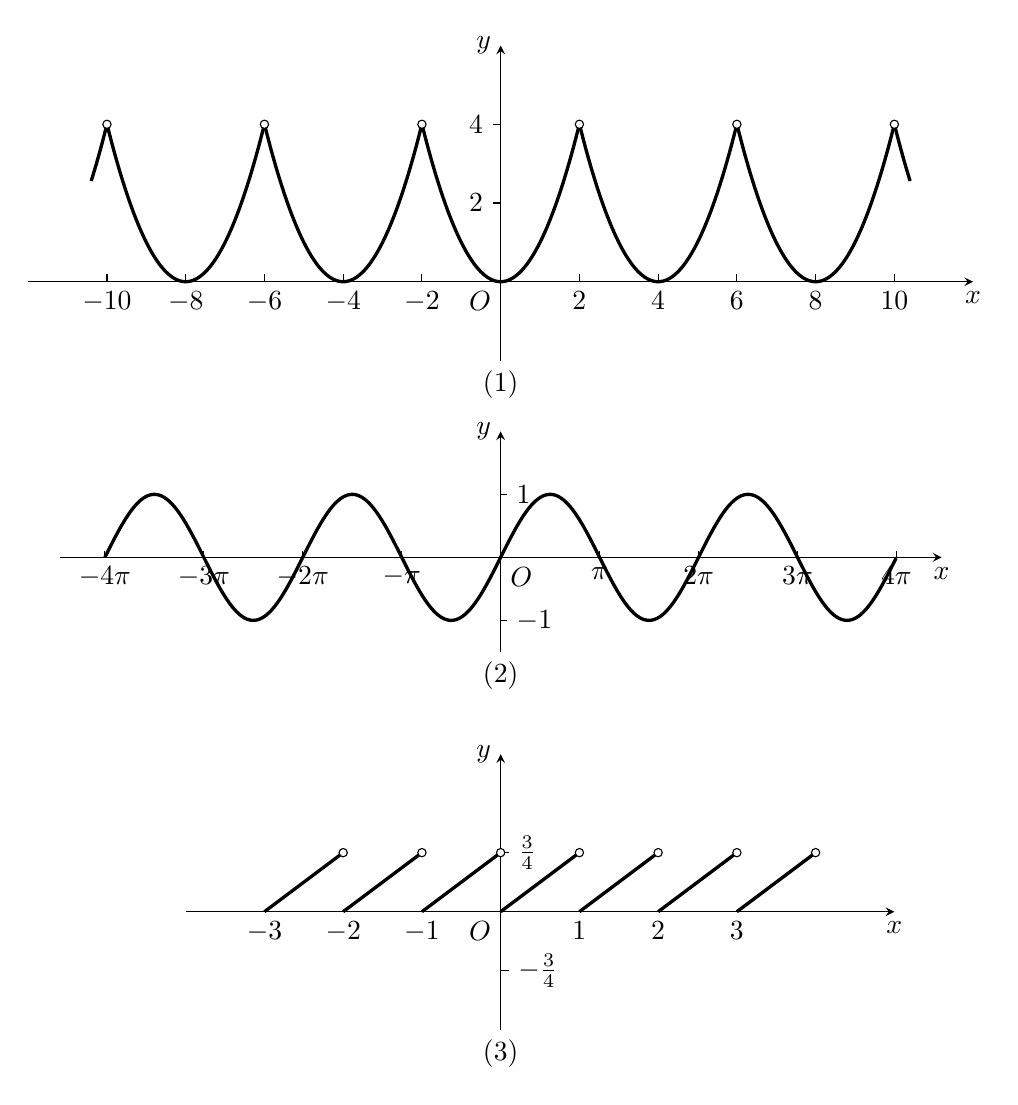
\begin{tikzpicture}[>=stealth]
\begin{scope}
\draw[->](-6,0)--(6,0)node[below]{$x$};
\draw[->](0,-1)node[below]{(1)}--(0,3)node[left]{$y$};
\foreach \x in {-10,-8,...,-2,2,4,...,10}
{
    \draw(\x/2, 0)node[below]{$\x$}--(\x/2,.1);
}
\foreach \x in {2,4}
{
    \draw(-.1,\x/2)node[left]{$\x$}--(0,\x/2);
}
\node[below left]{$O$};
\foreach \y in {-4,-2,...,4}
{
    \draw[domain=-1:1, very thick, smooth]plot(\x+\y, 2*\x*\x);
}
\draw[domain=-1:-.8, very thick, smooth]plot(\x+6, 2*\x*\x);
\draw[domain=.8:1, very thick, smooth]plot(\x-6, 2*\x*\x);
\foreach \x in {-5,-3,-1,...,5}
{
    \draw[fill=white](\x,2) circle(1.5pt);
}

\end{scope}    
\begin{scope}[yshift=-3.5cm, scale=.8]
\draw[->](-7,0)--(7,0)node[below]{$x$};
\draw[->](0,-1.5)node[below]{(2)}--(0,2)node[left]{$y$};
\draw[domain=-2*pi:2*pi, very thick, smooth, samples=1000]plot(\x, {sin(2*\x r)});
\node[below right]{$O$};
\foreach \x in {-4,-3,-2,2,3,4}
{
    \draw(\x*pi/2,0)node[below]{$\x\pi$}--(\x*pi/2,0.1);
}
\draw(pi/2,0)node[below]{$\pi$}--(pi/2,0.1);
\draw(-pi/2,0)node[below]{$-\pi$}--(-pi/2,0.1);
\foreach \x in {-1,1}
{
    \draw(0,\x)--(.1,\x)node[right]{$\x$};
}


\end{scope}   
\begin{scope}[yshift=-8cm]
    \draw[->](-4,0)--(5,0)node[below]{$x$};
    \draw[->](0,-1.5)node[below]{(3)}--(0,2)node[left]{$y$};
\foreach \x in {-3,-2,...,3}
{
    \draw[very thick](\x, 0)--(\x+1,.75);
}
\foreach \x in {1,2,3}
{
    \node at (\x,0)[below]{$\x$};
    \node at (-\x,0)[below]{$-\x$};
}
\node[below left]{$O$};

\draw (0,.75)--(.1,.75)node [right]{$\frac{3}{4}$};
\draw (0,-.75)--(.1,-.75) node[right]{$-\frac{3}{4}$};

\foreach \x in {-3,-2,...,3}
{
    \draw[fill=white](\x+1,.75)circle(1.5pt);
}

\end{scope}   
\end{tikzpicture}
    \caption{}
\end{figure}

细致地分析三个图象,可以发现:

每个图象都可以“平分”成大小、形状完全相同的无数段。用$y$随$x$变化的规律可以描述成:在定义域$D$中,对任何一个自变量$x$,当它增加一个固定的常数$T$[如对$f_1(x)$,$T_1=4$;对$f_2(x)$,$T_2=2\pi$;对$f_3(x)$,$T_3=1$]以后,函数值都重复出现(周而复始).

把这种共同特征,用符号语言给予精确化就有

\begin{thm}
 {定义} 对于函数$y=f(x),\; x\in D$,若存在常数$T\ne 0$,使任取$x\in D$,都有
\begin{equation}
     f(x)=f(x+T)\tag{*}
\end{equation}
称$y=f(x),\; x\in D$为\textbf{周期函数},$T$称为它的\textbf{周期}。   
\end{thm}

\begin{note}
\begin{enumerate}
    \item 定义中:不为零的常数T满足的条件是:
“任取$x\in D$,都有$f(x)=f(x+T)$”.

应注意所谓“任取$x\in D$”就是可以取遍$D$中的每一个$x$。由此可以看出,“周期性”是函数在$D$上的整体性质。由(*)还可以看出,$D$不能是有限区间(至少在一个方向是无限的)。
\item 定义的实质:
(*)表明,对于常数$T\ne 0$,定义域$D$中的任何一个自变量$x$与$x+T$对应的函数值都相等。这正是函数值周而复始的根源。由此可见,只要弄清了$f(x)$在一个周期内的性质,那么,$f(x)$在其他周期内的性质由(*)式可以直接推断出来。这将给函数性质的研究带来极大的方便。
\item 欲判断一个函数是否为周期函数,在于是否存在如上的常数$T$。若存在,就是周期函数;若不存在,就不是周期函数。根据这个定义可以得出:问1给出的三个函数都是周期函数,且它们的周期依次是$4,\; 2\pi,\;1$.
\item 对于不同的周期函数,$T$的值可能不等[如上述的$f_1(x)$的$T_1=1$,$f_2(x)$的$T_2=2\pi$……],即使对于同一个周期函数,$T$的值也不唯一。事实上,若$T$是$f(x)$的周期,则$2T,3T,\ldots kT\; (k\in\N)$都是$f(x)$的周期(这一点从$T$满足的性质可以推得。从上述三个函数的图象也可以直观地看出来).
\end{enumerate}
\end{note}

\begin{thm}
    {思考题}  $y=\sin x\; (x\in\R)$是周期函数吗?试述理由。
\end{thm}

现在,研究三角函数的周期性。

\subsection{$\sin x$、$\cos x$}

$\because\quad \sin ( x+ 2k\pi ) = \sin x, \quad \cos(x+2k\pi)=\cos x$ 
($x\in \R$, \; $k\in \Z$, 且$k\neq 0$).

$\therefore\quad \sin x$、$\cos x$都是周期函数,它们的周期
$$T=2k\pi\; (k\in \Z,\; k\neq0).$$

\subsection{$\tan x$、$\cot x$}

$\because\quad \tan(x+k\pi)=\tan x,\quad (x\in\mathbb{R}, \text{ 且 } x\neq\frac\pi2+k\pi,\; k\in \Z)$

$\cot ( x+ k\pi ) = \cot x, \; ( x\in \R, \text{ 且 }x\neq k\pi,\; k\in \Z)$

$\therefore\quad \tan x, \cot x$也都是周期函数,其周期$T= k\pi\; ( k\in \Z,\; k\ne 0)$.


由上可见,对$y=\sin x$来说,它的周期有$\pm2\pi,\pm4\pi,\pm6\pi,\ldots$.其中,具有代表性的(也是最常用的)是$2\pi$。它是$\sin x$的所有正的周期中最小的一个,称为\textbf{最小正周期},记为$T_{\text{最小正}}=2\pi$. 今后,求一个周期函数的周期,只要写出它的最小正周期即可。

\begin{example}
    证明:$2\pi$是$f(x)=\sin x$的最小正周期。
\end{example}

\begin{analyze}
    由于$\pm2\pi,\pm4\pi, \ldots$都是$\sin x$的周期(上面已经证明),以下只须证任何小于$2\pi$的正数都不是$\sin x$的周期。用反证法。
\end{analyze}

\begin{proof}
    设$\ell$是$\sin x$的周期,且$0<\ell<2\pi$,则任取$x\in\R$,都有$\sin(x+\ell)=\sin x$. 
    
由此,$2\cos\left(x+\frac{\ell}{2}\right)\sin\frac{\ell}{2}=0$对一切$x\in\R$都 成立。

又$\because\quad \cos\left(x+\frac{\ell}{2}\right)\not\equiv 0$

$\therefore\quad \sin\frac{\ell}{2}=0$

但由于$0<\ell<2\pi$,所以 $\sin\frac{\ell}{2}\ne 0$,矛盾.

$\therefore\quad $题设不真,从而$\sin x$的最小正周期为$2\pi$.
\end{proof}

类似地可以 证明:\textbf{$\cos x$的最小 正周期也是$2\pi$,$\tan x$、$\cot x$的最小正周期是$\pi$.}


\begin{example}
用定义判断下列 函数 是否是周期函数?
\begin{multicols}{3}
\begin{enumerate}[(1)]
    \item $f_1(x)=5$
    \item $f_2(x)=2^{x}$
    \item $f_3(x)=\sin 2x$
\end{enumerate}
\end{multicols}
\end{example}

\begin{solution}
\begin{enumerate}[(1)]
    \item 设$T\ne 0$,$f_1(x)=5$,$f_1(x+T)=5$
    
    欲使$T$为$f_1(x)$的周期,应有
    $f(x+T)=f(x)$对一切$x\in\R$都成立. 即$5=5$对一切$x$都成立,这是显然的。
    
    $\therefore\quad f_1(x)=5$是周期函数(周期为任意非零实数)。
    \item 设$T\ne 0$, $f_2(x)=2^x$, $f_2(x+T)=2^{x+T}$。
    
    欲使$T$为$f_2(x)$的周期,应有
    $2^{x+T}=2^x$对一切$x\in \R$都成立。$\Rightarrow 2^T=1\Rightarrow T=0$,矛盾。
    
    $\therefore\quad f_2(x)=2^x$不是周期函数。
    \item 设$T\ne 0$, $f_3(x)=\sin2x$, 
    $f_3(x+T)=\sin2(x+T)$.

    欲使$T$为$f_3(x)$的周期,应使
    $\sin2(x+T)=\sin2x$对一切$x\in\R$都成立,

    由于
    $\sin(2x+2T)=\sin2x$等价于
    $$\sin(2x+2T)-\sin2x=2\cos(2x+T)\sin T=0$$
而$\cos(2x+T)\not\equiv 0$,要使上式对一切$x\in\R$成立,应使$\sin T=0$,这只要取$T=\pi$即可.

$\therefore\quad f_3(x)=\sin 2x$是周期 函数(周期 是$2\pi$).
\end{enumerate}
\end{solution}

\begin{note}
用这里的方法 可以 证明:$y=A\sin (\omega x+\varphi)$,$y=A\cos (\omega x+\varphi)$,$y=A\tan (\omega x+\varphi)$,$y=A\cot (\omega x+\varphi)$(其中$A\ne 0,\; \omega>0$)都 是周期函数.
\end{note}

\begin{example}
求下列周期函数的周期:
\begin{multicols}{2}
\begin{enumerate}[(1)]
    \item $f(x)=2\sin\left(\frac{x}{2}-\frac{\pi}{6}\right)$
    \item $f(x)=\tan\left(2x+\frac{\pi}{3}\right)$
\end{enumerate}
\end{multicols}    
\end{example}

\begin{solution}
\begin{enumerate}[(1)]
    \item $f(x)=2\sin\left(\frac{x}{2}-\frac{\pi}{6}\right)$, 设实数$T>0$, 有
\[f(x+T)=2\sin\left[\frac{1}{2}(x+T)-\frac{\pi}{6}\right]=2\sin\left(\frac{x}{2}+\frac{T}{2}-\frac{\pi}{6}\right)\]

欲使$T$为$f(x)$的周期,须对于任意的$x\in D$, 都有
\begin{equation}
\begin{split}
    2\sin\left(\frac{x}{2}-\frac{\pi}{6}\right)&=2\sin\left(\frac{x}{2}+\frac{T}{2}-\frac{\pi}{6}\right)\\
    &=2\sin\left(\frac{x}{2}-\frac{\pi}{6}+\frac{T}{2}\right)
\end{split}\tag{*}
\end{equation}
利用$\sin x$的周期为$2\pi$, 得$\frac T2= 2\pi \Rightarrow T= 4\pi$.

$\therefore\quad f(x)=2\sin\left(\frac{x}{2}-\frac{\pi}{6}\right)$的周期 为$4\pi$.

\item $f(x)=\tan\left(2x+\frac{\pi}{3}\right)$,设实数$T>0$,有
\[f(x+T)=\tan\left[2(x+T)+\frac{\pi}{3}\right]=\tan\left(2x+\frac{\pi}{3}+2T\right)\]
欲使$T$为$f(x)$的周期, 须对任意的$x\in D$, 都有
\[\tan\left(2x+\frac{\pi}{3}\right)=\tan\left(2x+\frac{\pi}{3}+2T\right)\]
利用$\tan x$的周期为$\pi$, 得 $2T=\pi \Rightarrow T=\frac{\pi}{2}$

$\therefore\quad f(x)=\tan\left(2x+\frac{\pi}{3}\right)$的周期为$\frac{\pi}{2}$.

\end{enumerate}
\end{solution}

\begin{example}
试求$f(x)=A\sin(\omega x+\varphi)$的周期 ($A\neq0,\; \omega\neq0$)。
\end{example}

\begin{solution}
设实数$T>0$, 有$f(x+T)=A\sin\left(\omega x+\varphi+\omega T\right)$.
欲使$T$为$f(x)$的周期,须对任意的$x\in D$, 都有
$$A\sin\left(\omega x+\varphi\right)=A\sin\left(\omega x+\varphi+\omega T\right)$$

由于$A\neq0$, $\sin x$的周期为$2\pi$,
\begin{itemize}
\item 当 $\omega>0$时,取$\omega T=2\pi\Rightarrow T=\frac{2\pi}\omega$,
\item 当$\omega<0$时,取$-\omega T=2\pi\Rightarrow T=\frac{2\pi}{-\omega}$,
\end{itemize}

$\therefore$ $T= \frac {2\pi }{| \omega | }$.
\end{solution}
    
\section*{习题四}
\begin{center}
    \bfseries A
\end{center}

\begin{enumerate}
    \item \begin{enumerate}[(1)]
        \item 等式$\sin(30^{\circ}+120^{\circ})=\sin30^{\circ}$是否成立?若此式成立,能否说$120^{\circ}$是正弦函数$y=\sin x$的周期?为什么?
        \item 等式$\sin(x-4\pi)=\sin x$是否对一切$x\in\R$都成立?若此式成立,能否说$-4\pi$是$\sin x$的周期?为什么?
        \item 对于问1中的$f_3(x)$,求$f_3(100)$、$f_3\left(10\frac{1}{2}\right)$.
    \end{enumerate}
    \item 证明:常数函数$y=C$是以任意非零实数为周期的周期函数。
    \item 利用基本三角函数的周期,求下列复合三角函数的周期:
\begin{multicols}{2}
\begin{enumerate}[(1)]
    \item $y= \sin 3x$
    \item $y= \cos\frac{x}{3}$
    \item $y= 3\sin\frac{x}{4}$
    \item $y= \sin\left(x+\frac{\pi}{10}\right)$
    \item $y= \cos\left(2x+\frac{\pi}{3}\right)$
    \item $y= \sqrt{3}\sin\left(\frac{x}{2}-\frac{\pi}{4}\right)$
    \item $y= \tan 2x$
\end{enumerate}
\end{multicols}
\end{enumerate}

\begin{center}
    \bfseries B
\end{center}

\begin{enumerate}\setcounter{enumi}{3}
    \item 同上题:
\begin{multicols}{2}
\begin{enumerate}[(1)]
    \item $y=\cot\left(x+\frac{\pi}{3}\right)$
    \item $y=5\tan\frac{x}{2}$
    \item $y=\tan(\omega x+\varphi)\quad (\omega\ne 0)$
\end{enumerate}
\end{multicols}
\end{enumerate}

\begin{center}
    \bfseries C
\end{center}
\begin{enumerate}\setcounter{enumi}{4}
    \item 证明 $y=\cos\sqrt{x}$不是周期函数.
\end{enumerate}

\section{正弦函数与余弦函数的图象}
利用三角函数线容易作出正弦函数与余弦函数的图象.

在$xOy$坐标系中,取$x$轴上任一点$O_1$为圆心作单位圆(图
3.12上半部分),从此圆与$x$轴的交点$A$起,把圆分成12等份(等份越多,作出的图象越精确),分点$A,P_1,P_2,P_3,\ldots, P_{11},P_{12}$依次对应的角为
$0,\frac{\pi}{6},\frac{2\pi}{6},\frac{3\pi}{6},\ldots,\frac{11\pi}{6},2\pi$。过诸分点分别作$y$轴和$x$轴的垂线,就可得到上述各角对应的正弦线和余弦线(例如$\VEC{O_1P_3}$就是角$\frac{\pi}{2}$的正弦线)。相应地,把$x$轴上从0到$2\pi$这一段($2\pi\approx 6.2828$)分成12等份(例如,从原点起向右第四个点,就对应角为$\frac{\pi}{2}$的点)。再把角$x$对应的正弦线向右平移到起点与$x$轴上的$x$点重合的位置(例如,把正弦线$\VEC{O_1P_3}$平移到起点为$Ox$轴上$\frac{\pi}{2}$点处),最后用光滑曲线把这些正弦线的终点连接起来,就得到正 弦函数$y=\sin x,\; x\in [0,2\pi]$的图象。

\begin{figure}[htp]
    \centering
\begin{tikzpicture}[>=stealth]
\draw[->](-2,0)--(9,0)node[below]{$x$};
\draw[->](2,-1.5)--(2,2)node[left]{$y$};


\draw[thick] (0,0)node[below]{$O_1$} circle (1);
\foreach \x in {1,2,...,12}
{
    \tkzDefPoint(30*\x:1){P\x}
    \draw[thick](0,0)--(P\x);
}
\draw[domain=0:2*pi, samples=100, very thick, smooth]plot(\x+2, {sin(\x r)});

\foreach \x in {1,2,3,4,5,7,8,9,10,11}
{
    \draw(\x*pi/6+2, 0)--(\x*pi/6+2, {sin(30*\x)});
    \draw[dashed](30*\x:1)--(\x*pi/6+2, {sin(30*\x)});
}

\foreach \x in {7,8,9,10,11,12}
{
    \node at (\x*pi/6+2, {sin(30*\x)})[below]{$P_{\x}$};
}
\foreach \x in {1,2,3,4,5,6}
{
    \node at (\x*pi/6+2, {sin(30*\x)})[above]{$P_{\x}$};
}
\foreach \x in {1,2}
{
    \node at (P\x)[above right]{$P_{\x}$};
}
\foreach \x in {4,5,6}
{
    \node at (P\x)[above left]{$P_{\x}$};
}
\node at (P3)[above]{$P_3$};
\node at (1,0)[above right]{$A$};
\node at (P9)[below]{$P_9$};
\foreach \x in {7,8}
{
    \node at (P\x)[below left]{$P_{\x}$};
}
\foreach \x in {10,11,12}
{
    \node at (P\x)[below right]{$P_{\x}$};
}
\node at (2,0)[below right]{$O$};
\node at (2,1)[above left]{1};
\node at (2,-1)[below left]{$-1$};
\node at (2+pi/2,0)[below]{$\frac{\pi}{2}$};
\node at (2+pi,0)[below left]{$\pi$};
\node at (2+pi*1.5,0)[above]{$\frac{3\pi}{2}$};
\node at (2+pi*2,0)[above]{$2\pi$};


\draw[thick](-1.5,-5.5)node[above]{$\ell$}--(0,-4)--(1.5,-2.5);


\draw[->](-2,-4)--(9,-4)node[below]{$x$};
\draw[->](2,-2-4)--(2,2-4)node[left]{$y$};
\draw[domain=0:2*pi, samples=100, very thick, smooth]plot(\x+2, {cos(\x r)-4});
\foreach \x in {1,2,4,5,6,7,8,10,11,12}
{
    \draw(\x*pi/6+2, -4)--(\x*pi/6+2, {cos(30*\x)-4});
}

\draw[dashed](0:1)--(1,-4+1)--(2*pi+2, {cos(30*0)-4});
\draw[dashed](30:1)--(1.732/2,-4+1.732/2)--(11*pi/6+2, {cos(30*11)-4});
\draw[dashed](60:1)--(1/2,-4+1/2)--(10*pi/6+2, {cos(30*10)-4});
\draw[dashed](90:1)--(0,-4+0);
\draw[dashed](120:1)--(-1/2,-4-1/2)--(8*pi/6+2, {cos(30*8)-4});
\draw[dashed](150:1)--(-1.732/2,-4-1.732/2)--(7*pi/6+2, {cos(30*7)-4});
\draw[dashed](180:1)--(-1,-4-1)--(pi+2, {cos(30*6)-4});

\draw[dashed](1,-3)node[right]{$A'$}--(1,-4)node[below]{$A$};
\node at (2,-3)[above left]{$A$};
\node at (2+pi/2,-4)[above right]{$\frac{\pi}{2}$};
\node at (2+pi,-4)[above]{$\pi$};
\node at (2+pi*1.5,-4)[below right]{$\frac{3\pi}{2}$};
\node at (2+pi*2,-4)[below]{$2\pi$};
\node at (2,-4)[below left]{$O$};


\foreach \x in {3,4,5,6,7,8}
{
    \node at (\x*pi/6+2, {cos(30*\x)-4})[below]{$P_{\x}$};
}
\foreach \x in {1,2,9,10,11,12}
{
    \node at (\x*pi/6+2, {cos(30*\x)-4})[above]{$P_{\x}$};
}
\node at (0,-4)[below right]{$O_1$};

\draw(0.35,-4) arc (0:45:.35)node[right]{$\tfrac{\pi}{4}$};

\node at (2,-3)[above right]{1};
\node at (2,-5)[below right]{$-1$};

\node at (6,1.8){$y=\sin x\quad x\in[0,2\pi]$};
\node at (6,1.8-4){$y=\cos x\quad x\in[0,2\pi]$};


\end{tikzpicture}
    \caption{}
\end{figure}




为了作出余弦函数$y=\cos x,\; x\in [0,2\pi]$的图象,我们把坐标系向下平移(图3.12的下半部分),过点$O_1$作与$x$轴成角$\frac{\pi}{4}$的直线$\ell$,又过余弦线$\VEC{O_1A}$的终点$A$作$x$轴的垂线与$\ell$相交于$A'$,这样得到的与$\VEC{Oy}$同向,且长度为$|\VEC{O_1A}|$的有向线段$\VEC{AA'}$,相当于把余弦线$\VEC{O_1A}$“竖立”起来了。同样的方法,将其余的余弦线都“竖立”起来。再将它们向右平移,使角$x$对应的余弦线的起点与$x$轴上的点$x$重合,最后用光滑曲线把这些竖立起来的有向线段的终点连接起来,就得到余弦函数$y=\cos x,\; x\in[0,2\pi]$的图象。

因为正弦函数和余弦函数的周期都是$2\pi$,所以,图3.12中实际上画出了它们一个周期内的图象。这时,只要分别向左、右一个周期一个周期地延展出去,就可以得出$y=\sin x\; (x\in\R)$及$y=\cos x\; (x\in\R)$的图象(图3.13)。

正弦函数$y=\sin x\; (x\in\R)$和余弦函数$y=\cos x\; (x\in\R)$的图象分别叫做\textbf{正弦曲线}和\textbf{余弦曲线}.

观察正弦曲线与余弦曲线(图3.13),可以看出它们体
现出了前面研究过\textbf{正弦与余弦函数的性质}。

\begin{enumerate}[(1)]
\item 定义域:
$y=\sin x$, $y=\cos x$的定义域都是$\R$。
\item 值域:
$y=\sin x$, $y=\cos x$的值域都是$[-1,1]$.
\item 周期性:
$y=\sin x$, $y=\cos x$都是周期函数,$2\pi$是它们的最小正周期。
\item 单调性:
\begin{itemize}
    \item 对于$y=\sin x\; (x\in\R)$, 
增区间是$\left[-\frac{\pi}{2}+2k\pi,\; \frac{\pi}{2}+2k\pi\right],\; k\in\Z$,减区间是$\left[\frac{\pi}{2}+2k\pi,\; \frac{3\pi}{2}+2k\pi\right],\; k\in\Z$
\item 对于$y=\cos x\; (x\in\R)$, 
增区间是$\left[\pi+2k\pi,\; 2\pi+2k\pi\right],\; k\in\Z$,减区间是$\left[0+2k\pi,\; \pi+2k\pi\right],\; k\in\Z$
\end{itemize}

\item 奇偶性:
\begin{itemize}
    \item $y=\sin x\; (x\in\R)$是奇函数(图象关于原点对称)
    \item $y=\cos x\; (x\in\R)$是偶函数(图象关于$y$轴对称)
\end{itemize}
\end{enumerate}

\begin{figure}[htp]
    \centering
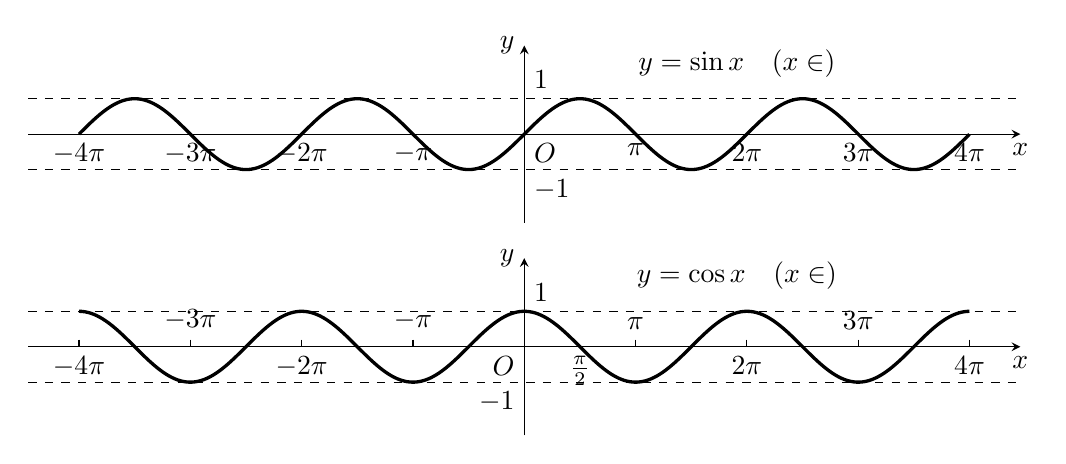
\begin{tikzpicture}[>=stealth, scale=.45]
\begin{scope}
    \draw[->](-14,0)--(14,0)node[below]{$x$};
    \draw[->](0,-2.5)--(0,2.5)node[left]{$y$};
\foreach \x in {-1,1}
{
    \draw[dashed](-14,\x)--(14,\x);
}
\draw[very thick, domain=-4*pi:4*pi, samples=300]plot(\x, {sin(\x r)});
\foreach \x in {2,3,4,-2,-3,-4}
{
    \node at (\x*pi,0)[below]{$\x\pi$};
}
\node at (pi,0)[below]{$\pi$}; \node at (-pi,0)[below]{$-\pi$};
\node at (0,1)[above right]{1};
\node at (0,-1)[below right]{$-1$};
\node[below right]{$O$};
\node at (6,2){$y=\sin x\quad (x\in\R)$};


\end{scope}
\begin{scope}[yshift=-6cm]
    \draw[->](-14,0)--(14,0)node[below]{$x$};
    \draw[->](0,-2.5)--(0,2.5)node[left]{$y$};
\foreach \x in {-1,1}
{
    \draw[dashed](-14,\x)--(14,\x);
}
\draw[very thick, domain=-4*pi:4*pi, samples=300]plot(\x, {cos(\x r)});
\foreach \x in {2,4,-2,-4}
{
    \draw(\x*pi,.2)--(\x*pi,0)node[below]{$\x\pi$};
}
\foreach \x in {3,-3}
{
    \draw(\x*pi,.2)node[above]{$\x\pi$}--(\x*pi,0);
}
\draw(1*pi,.2)node[above]{$\pi$}--(1*pi,0);
\draw(-1*pi,.2)node[above]{$-\pi$}--(-1*pi,0);
\node at (0,1)[above right]{1};
\node at (0,-1)[below left]{$-1$};
\node[below left]{$O$};
\node at (pi/2,0)[below]{$\frac{\pi}{2}$};
\node at (6,2){$y=\cos x\quad (x\in\R)$};
\end{scope}
\end{tikzpicture}
    \caption{}
\end{figure}

上面介绍的用三角函数线作图象的方法基本上是几何方法。我们还可以用描点法(代数方法)来作图象。特别,当精度要求不太高时,选择图象上的几个特殊点(关键点)来描迹是简单易行而且经常使用的。
    
对$y=\sin x,\; x\in[0,2\pi]$而言,下列五个点:
\[(0,0),\quad \left(\frac{\pi}{2},\; 1\right),\quad (\pi,0),\quad \left(\frac{3\pi}{2},\; -1\right) \quad (2\pi,0)\]
无论对函数性质的研究,还是对正确作图象,都起着关键的作用。事实上,这五个点中有三个是函数的零点(函数值为零的点),一个是最大值点(函数值在该点取到最大值),一个是最小值点(图3.13)。在一个周期内,若这五个点的位置确定了,那么,整个图象就基本确定了。因此,作图时,常常先描出这五个点,然后再用光滑曲线把它们连结起来,就得到了这个周期内的正弦函数的简图。这种用上述五个关键点描绘正弦函数简图的方法通常称为“\textbf{五点法}”。

对$y=\cos x,\; x\in[0,2\pi]$,通常也用“五点法”作简图。五个关键点选择为:
\[(0,1),\quad \left(\frac{\pi}{2},\; 0\right),\quad (\pi,-1),\quad \left(\frac{3\pi}{2},\; 0\right) \quad (2\pi,1)\]
其中,有两个零点,两个最大值 点,一个最小值点(图3.13).

\begin{example}
用“五点法”作下列函数的简图:
\begin{enumerate}[(1)]
    \item $y=1+\sin x,\quad x\in[0,2\pi]$
    \item $y=-\cos x,\quad x\in[0,2\pi]$
\end{enumerate}
\end{example}

\begin{solution}
\begin{enumerate}[(1)]
    \item 列表:(先填第一、二行,再填第三行)
\begin{center}
\begin{tabular}{c|ccccc}
\hline
$x$ & 0&$\frac{\pi}{2}$& $\pi$& $\frac{3\pi}{2}$& $2\pi$\\[1.5ex]
\hline
$\sin x$& 0&1&0&$-1$&0\\
$y=1+\sin x$& 1&2&1&0&1\\
\hline
\end{tabular}
\end{center}

在$xOy$坐标 系中,描点,作图(图3.14).

\begin{figure}[htp]
    \centering
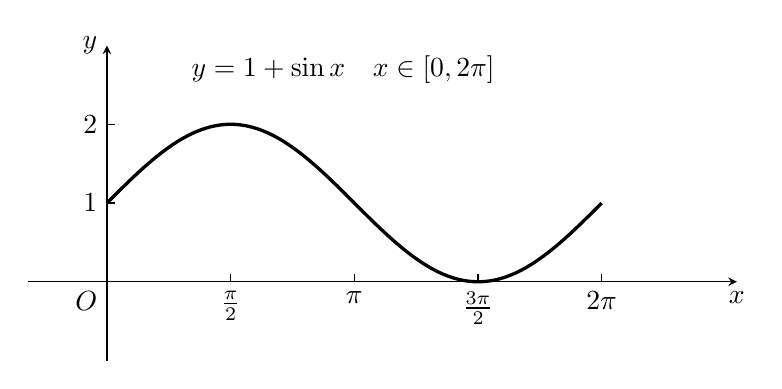
\begin{tikzpicture}[>=stealth]
    \draw[->](-1,0)--(8,0)node[below]{$x$};
    \draw[->](0,-1)--(0,3)node[left]{$y$};
\draw[domain=0:2*pi, samples=100, smooth, very thick]plot(\x, {sin(\x r)+1});
\foreach \x in {1,2}
{
    \draw(0,\x)node[left]{\x}--(.1,\x);
}
\node [below left]{$O$};

\foreach \x/\y in {1/\frac{\pi}{2},2/\pi,3/\frac{3\pi}{2},4/2\pi}
{
    \draw(\x*pi/2,0)node[below]{$\y$}--(\x*pi/2,0.1);
}
\node at (3,2.7){$y=1+\sin x\quad x\in[0,2\pi]$};
\end{tikzpicture}
    \caption{}
\end{figure}

\item 列表:
\begin{center}
\begin{tabular}{c|ccccc}
\hline
$x$ & 0&$\frac{\pi}{2}$& $\pi$& $\frac{3\pi}{2}$& $2\pi$\\[1.5ex]
\hline
$\cos x$& 1&0&$-1$&0&1\\
$y=-\cos x$& $-1$&0&1&0&$-1$\\
\hline
\end{tabular}
\end{center}

在$xOy$坐标 系中,描点,作图(图3.15).

\begin{figure}[htp]
    \centering
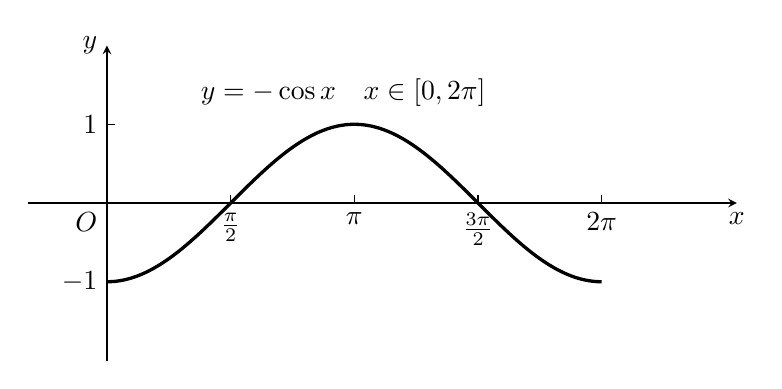
\begin{tikzpicture}[>=stealth]
    \draw[->](-1,0)--(8,0)node[below]{$x$};
    \draw[->](0,-2)--(0,2)node[left]{$y$};
\draw[domain=0:2*pi, samples=100, smooth, very thick]plot(\x, {-cos(\x r)});
\foreach \x in {1,-1}
{
    \draw(0,\x)node[left]{$\x$}--(.1,\x);
}
\node [below left]{$O$};

\foreach \x/\y in {1/\frac{\pi}{2},2/\pi,3/\frac{3\pi}{2},4/2\pi}
{
    \draw(\x*pi/2,0)node[below]{$\y$}--(\x*pi/2,0.1);
}
\node at (3,1.4){$y=-\cos x\quad x\in[0,2\pi]$};
\end{tikzpicture}
    \caption{}
\end{figure}
\end{enumerate}
\end{solution}

\begin{example}
用“五点法”作下列函数在一个周期内的简图:
\begin{multicols}{2}
\begin{enumerate}[(1)]
    \item $y=\sin 2x$
    \item $y=3\sin\left(2x+\frac{\pi}{4}\right)$
\end{enumerate}
\end{multicols}
\end{example}

\begin{solution}
\begin{enumerate}[(1)]
    \item 在$y=\sin 2x$中,设$t=2x$ \hfill(1)

则有
\begin{equation}
    y=\sin t \tag{2}
\end{equation}

(2)是基本的三角函数,因而,可用“五点法”的思想取出它的五个关键点(这只要设$t=0,\; \frac{\pi}{2},\;\pi,\;\frac{3\pi}{2},\; 2\pi$即可)。然后,据(1),再使,$(t,y)$变换成$(x,y)$. 列表如下:
\begin{center}
\begin{tabular}{c|ccccc}
\hline
$x$ & 0&$\frac{\pi}{2}$& $\pi$& $\frac{3\pi}{2}$& $2\pi$\\[1.5ex]
\hline
$x=\frac{t}{2}$& 0&$\frac{\pi}{4}$&$\frac{\pi}{2}$&$\frac{3\pi}{4}$&$\pi$\\[1.5ex]
$y=\sin t$& $0$&1&0&$-1$&$0$\\
\hline
\end{tabular}
\end{center}
(注:这个表,先填第一、三行,后填第二行)

在$xOy$坐标 系中,描点,作图(图3.16).

\item 在$y=3\sin\left(2x+\frac{\pi}{4}\right)$中,设$t=2x+\frac{\pi}{4}$\hfill(1)

则有
\begin{equation}
    y=3\sin t \tag{2}
\end{equation}

列表:(先填第一、三行,后填第二行)
\begin{center}
\begin{tabular}{c|ccccc}
\hline
$t$ & 0&$\frac{\pi}{2}$& $\pi$& $\frac{3\pi}{2}$& $2\pi$\\[1.5ex]
\hline
$x=\frac{t-\frac{\pi}{4}}{2}$& $-\frac{\pi}{8}$&$\frac{\pi}{8}$&$\frac{3\pi}{8}$&$\frac{5\pi}{8}$&$\frac{7\pi}{8}$\\[1.5ex]
$y=3\sin t$& $0$&3&0&$-3$&$0$\\[1.5ex]
\hline
\end{tabular}
\end{center}

在$xOy$坐标系中,描点,作图(图3.17).
\end{enumerate}

\noindent
\begin{minipage}{.45\textwidth}
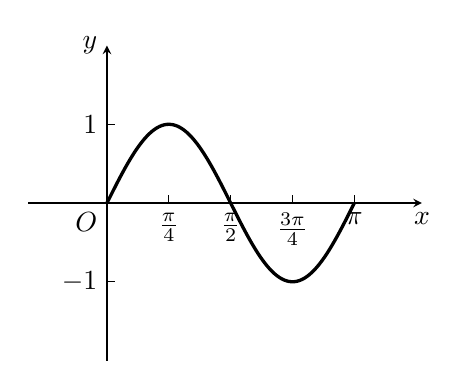
\begin{tikzpicture}[>=stealth]
    \draw[->](-1,0)--(4,0)node[below]{$x$};
    \draw[->](0,-2)--(0,2)node[left]{$y$};
\draw[domain=0:pi, samples=100, smooth, very thick]plot(\x, {sin(2*\x r)});
\foreach \x in {1,-1}
{
    \draw(0,\x)node[left]{$\x$}--(.1,\x);
}
\node [below left]{$O$};

\foreach \x/\y in {1/\frac{\pi}{4},2/\frac{\pi}{2},3/\frac{3\pi}{4},4/\pi}
{
    \draw(\x*pi/4,0)node[below]{$\y$}--(\x*pi/4,0.1);
} 

\end{tikzpicture}    
\captionof{figure}{}
\end{minipage}\hfill
\begin{minipage}{.45\textwidth}
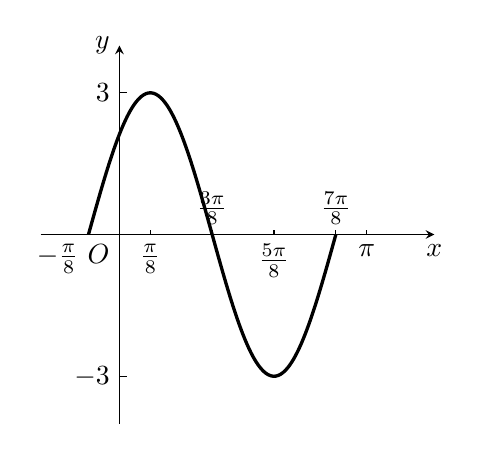
\begin{tikzpicture}[>=stealth, yscale=.6]
    \draw[->](-1,0)--(4,0)node[below]{$x$};
    \draw[->](0,-4)--(0,4)node[left]{$y$};
\draw[domain=0:pi, samples=100, smooth, very thick]plot(\x-pi/8, {3*sin (2*\x r)});
\foreach \x in {3,-3}
{
    \draw(0,\x)node[left]{$\x$}--(.1,\x);
}
\node [below left]{$O$};

\foreach \x/\y in {1/\frac{\pi}{8},3/\frac{5\pi}{8}}
{
    \draw(\x*pi/4-pi/8,0)node[below]{$\y$}--(\x*pi/4-pi/8,0.1);
}
\foreach \x/\y in {2/\frac{3\pi}{8},4/\frac{7\pi}{8}}
{
    \draw(\x*pi/4-pi/8,0)node[above]{$\y$}--(\x*pi/4-pi/8,0.1);
}
\draw(pi,0)node[below]{$\pi$}--(pi,0.1);
\node at (-pi/8,0)[below left]{$-\frac{\pi}{8}$};
\end{tikzpicture}    
\captionof{figure}{}
\end{minipage}
\end{solution}

\begin{thm}
    {思考题} 用五点法如何作$y=\sin2x,\; x\in\left[\frac{\pi}{4},\; \frac{3\pi}{4}\right]$的简图?
\end{thm}

\begin{example}
    求下列函数的最大值与最小值,并指出当$x$为何值时,函数取到最大(小)值:
\begin{multicols}{2}
\begin{enumerate}[(1)]
    \item $f_1(x)=\cos x+2$
    \item $f_2(x)=\sin 2x$
    \item $f_3(x)=A\sin x\quad (A\ne 0)$
\end{enumerate}
\end{multicols}
\end{example}

\begin{solution}
\begin{enumerate}[(1)]
    \item 当$\cos x$取最大值时,$f_1(x)$的值为最大,

$\therefore\quad$ 当$x \in \{ x\mid x= 2k\pi, \; k\in \Z\}$时,$f_1(x)$的 最大值
为$1+2=3$;

当$\cos x$取最小值时,$f_1(x)$的值为最小,

$\therefore\quad $ 当 $x\in \{ x\mid x= \pi + 2k\pi,\; k\in \Z\}$时,$f_1(x)$的最小
值为$-1+2=1$.

\item 当$2x=\frac{\pi}{2}+2k\pi\; (k\in \Z)$时,$f_{2}(x)$的值最大,

$\therefore\quad x\in \left\{ x\Big|  x= \frac \pi 4+ k\pi,\; k\in \Z\right\}$时,$f_2(x)$取最大值1, 

当$2x=-\frac{\pi}{2}+2k\pi\; (k\in \Z)$时,$f_2(x)$的值最小,

$\therefore\quad$ 当$x\in \left\{ x\Big| x= - \frac \pi 4+ k\pi,\;  k\in \Z\right\}$时,$f_{2}( x)$ 取最小值$-1$.
\item  若$A>0$时,
\begin{itemize}
    \item 当$x=\frac{\pi}{2}+2k\pi\; (k\in \Z)$时,$f_{3}(x)$取最大值$A$;
    \item 当$x=-\frac{\pi}{2}+2k\pi\; (k\in \Z)$时, $f_3(x)$取最小值$-A$.
\end{itemize}

若$A<0$时,
\begin{itemize}
    \item 当$x=-\frac{\pi}{2}+2k\pi\; \left(k\in \Z\right)$时,$f_{3}(x)$取最大值$-A$;
    \item 当$x=\frac{\pi}{2}+2k\pi\; (k\in \Z)$时,$f_3(x)$ 取最小值$A$.
\end{itemize}
\end{enumerate}
\end{solution}

\begin{example}
    若$\cos x=\frac{a}{a-2}$,求$a$的取值范围.
\end{example}

\begin{analyze}
这是涉及余弦函数 值域 的问题.
\end{analyze}

\begin{solution}
$\because\quad \cos x\in[-1,1]$,要使原式有意义,必须

$\therefore\quad -1\le \frac{a}{a-2}\le 1$\hfill(1)

\[\begin{split}
(1)\Longleftrightarrow \begin{cases}
    \frac{a}{a-2}+1\ge 0\\
    \frac{a}{a-2}-1\le 0
\end{cases}&\Longleftrightarrow \begin{cases}
    \frac{2a-2}{a-2}\ge 0\\ 
    \frac{2}{a-2}\le 0
\end{cases}\\
&\Longleftrightarrow \begin{cases}
   2(a-1)(a-2)>0\;\text{或}\; a=1\\ 
    {a-2}< 0
\end{cases}\\
&\Longleftrightarrow \begin{cases}
    a<1\; \text{或}\; a>2\quad \;{或}\; a=1\\ 
    a<2
\end{cases}
\end{split}\]

$\therefore\quad a\le 1$
\end{solution}

\section*{习题五}
\begin{center}
    \bfseries A
\end{center}
\begin{enumerate}
    \item 用五点法作出下列函数在一个周期内的简图:
\begin{multicols}{2}
\begin{enumerate}[(1)]
    \item $y=\sin 4x$
    \item $y=2\sin \frac{1}{3}x$
    \item $y=4\sin\left(x-\frac{\pi}{3}\right) $
    \item $y=\sin \left(2x+\frac{\pi}{6}\right)$
    \item $y=5\sin\left(\frac{1}{2}x+\frac{\pi}{6}\right) $
    \item $y=\frac{1}{2}\sin \left(3x-\frac{\pi}{4}\right)$
\end{enumerate}
\end{multicols}
\item 用五点法作函数$y=3\sin\left(3x-\frac{\pi}{3}\right),\; x\in[0,\pi]$的简
图,并根据简图写出它的减区间。
\item 当$x$为哪些值时,下列函数取得最大(小)值,并指出最大(小)值是多少:
\begin{multicols}{2}
\begin{enumerate}[(1)]
    \item $y=2\sin x$
    \item $y=2-\cos\frac{x}{3}$
    \item $y=-5\sin x$
    \item $y=1-\frac{1}{2}\cos x$
    \item $y=3\sin\left(x+\frac{\pi}{3}\right)$
    \item $y=\frac{1}{2}\sin\left(\frac{1}{2}x+\frac{\pi}{4}\right)$
\end{enumerate}
\end{multicols}

\item 求下列函数的定义域与值域:
\begin{multicols}{2}
\begin{enumerate}[(1)]
    \item $y=4+\cos x$
    \item $y=2\cos\frac{x}{3}$
    \item $y=\sqrt{\sin x}$
    \item $y=\sqrt{1-\cos^2 x}$
\end{enumerate}
\end{multicols}
\end{enumerate}

\begin{center}
    \bfseries B
\end{center}

\begin{enumerate}\setcounter{enumi}{4}
    \item 要使下式有意义,求$a$的取值范围:$$\sec x=\frac{3a+2}{2-3a}$$
\end{enumerate}

\section{用几何变换的方法作函数的图象}
本节是对已学知识的复习与补充。课题是:根据已知函数
\begin{equation}
 y=f(x)\tag{*}   
\end{equation}
的图象,用几何变换的方法,作与$f(x)$密切相关的下列一些
新函数的图象。

\subsection{$y=f(x)+m$}
欲作函数$y=f(x)+m$的图象,只须把$y=f(x)$的图象作\textbf{纵向平移}(上移$m$个单位,见图3.18),即使$y=f(x)$图象上的每个点$(x,y)\to (x,y+m)$。

\begin{figure}[htp]
    \centering
\begin{tikzpicture}[>=stealth]
\draw[->](-2,0)--(4,0)node[below]{$x$};
\draw[->](0,-1)--(0,3)node[left]{$y$};
\draw[domain=-1.7:2.75, smooth, samples=100, very thick]plot(\x, {-sin(1.5*(\x-.5) r)+.5})node[right]{$y=f(x)$};
\draw[domain=-1.7:2.75, smooth, samples=100, dashed]plot(\x, {-sin(1.5*(\x-.5) r)+1.5})node[above]{$y=f(x)+m\quad (m>0)$};
\node[below left]{$O$};
\tkzDefPoints{-1/1.27/P, -1/2.27/P'}
\draw[fill](P)circle(1.5pt);
\draw[fill](P')circle(1.5pt);
\node at (P)[below right]{$P(x,y)$};
\node at (P')[above left]{$P'(x,y+m)$};

\end{tikzpicture}
    \caption{}
\end{figure}




\subsection{$y=f(x+m)$}
欲作$y=f(x+m)$的图象,只须把$y=f(x)$的图象作\textbf{横向平移}(左移$m$个单位,见图3.19),即使$y=f(x)$图象上的每个点$(x,y)\to (x-m,y)$

变换的推导过程:设$P(a,b)\in $曲线$y=f(x)$, 则$b=f(a)$. 对于$y=f(x+m)$,当$x+m=a$时,$y=b\Longrightarrow x=a-m,\; y=b$, 
由此可得$(a-m,b)\in $曲线$y=f(x+m)$,从而
$(x,y)\to (x-m,y)$.

\begin{figure}[htp]
    \centering
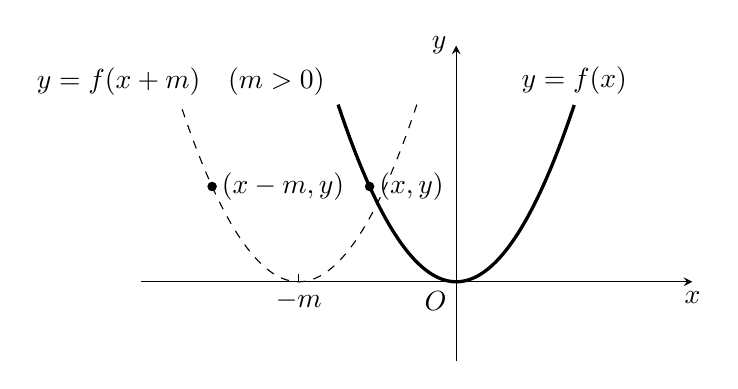
\begin{tikzpicture}[>=stealth]
\draw[->](-4,0)--(3,0)node[below]{$x$};
\draw[->](0,-1)--(0,3)node[left]{$y$};
\draw[domain=-1.5:1.5, smooth, samples=100, very thick]plot(\x, \x*\x)node[above]{$y=f(x)$};
\draw[domain=1.5:-1.5, smooth, samples=100, dashed]plot(\x-2, \x*\x)node[above]{$y=f(x+m)\quad (m>0)$};
\node[below left]{$O$};
\draw(-2,0)node[below]{$-m$}--(-2,.1);
\draw[fill](-1.1,1.21)node[right]{$(x,y)$} circle(1.5pt);
\draw[fill](-3.1,1.21)node[right]{$(x-m,y)$} circle(1.5pt);
\end{tikzpicture}
    \caption{}
\end{figure}


\subsection{$y=-f(x)$}
欲作$y=-f(x)$的图象,只须把(*)的图象作\textbf{$x$轴的对称变换}(图3.20),即使(*)上的每个点$(x,y)\to (x,-y)$.

\noindent
\begin{minipage}{.45\textwidth}
\centering
\begin{tikzpicture}[>=stealth]
\draw[->](-1,0)--(3,0)node[below]{$x$};
\draw[->](0,-2)--(0,2)node[left]{$y$};
\node[below left]{$O$};
\draw[domain=-1.5:1.5, very thick, smooth, samples=100]plot(\x+1, \x*\x-.5)node[above]{$y=f(x)$};
\draw[domain=-1.5:1.5, dashed, smooth, samples=100]plot(\x+1, -\x*\x+.5)node[below]{$y=-f(x)$};
\tkzDefPoints{1/-.5/P', 1/.5/P}
\tkzDrawPoints[fill=black](P,P')
\node at (P)[above]{$P(x,y)$};
\node at (P')[below]{$P'(x,-y)$};


\end{tikzpicture}
\captionof{figure}{}
\end{minipage}\hfill
\begin{minipage}{.55\textwidth}
  \centering
\begin{tikzpicture}[>=stealth]
\draw[->](-2.5,0)--(2.5,0)node[below]{$x$};
\draw[->](0,-1.5)--(0,3)node[left]{$y$};
\node[above left]{$O$};
\draw[domain=-1.65:1.65, very thick, smooth, samples=100]plot(\x+.5, \x*\x-.5)node[above]{$y=f(x)$};
\draw[domain=1.65:-1.65, dashed, smooth, samples=100]plot(\x-.5, \x*\x-.5)node[above]{$y=f(-x)$};
\tkzDefPoints{1.5/.5/P, -1.5/.5/P'}
\tkzDrawPoints[fill=black](P,P')
\node at (P)[right]{$P(x,y)$};
\node at (P')[left]{$P'(-x,y)$};
\end{tikzpicture}
\captionof{figure}{}
\end{minipage}



\subsection{$y=f(-x)$}

欲作$y=f(-x)$的图象,只须把(*)的图象作\textbf{$y$轴的对称变换}(图3.21),即使(*)上的每个点$(x,y)\to (-x,y)$.

\subsection{$y=Af(x)\quad (A>0)$}

欲作$y=Af(x)$的图象,只须把(*)的图象作\textbf{纵向伸缩变换}(上、下都压向$x$轴,图3.22),即使(*)上的每个点$(x,y)\to (x,Ay)$.

\begin{figure}[htp]
    \centering
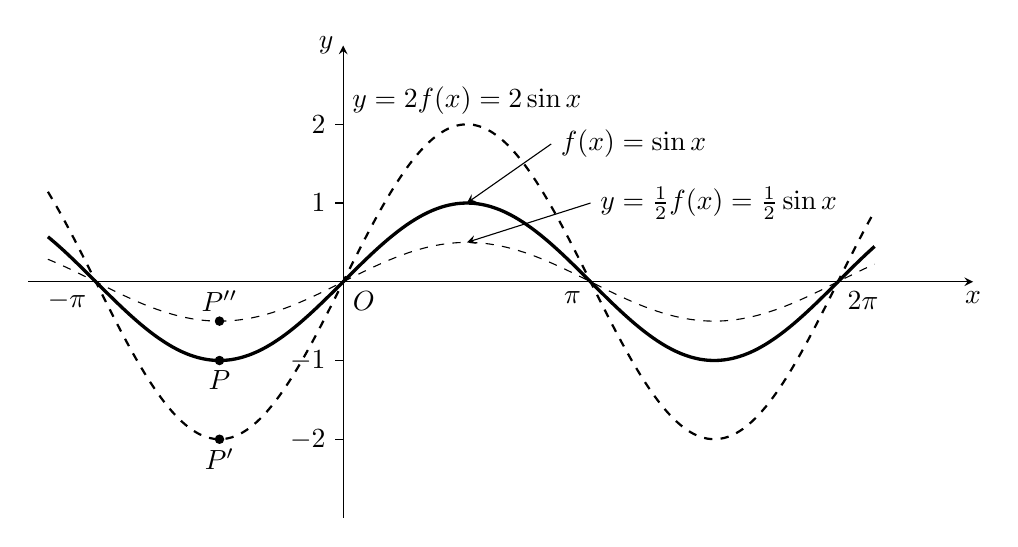
\begin{tikzpicture}[>=stealth]
    \draw[->](-4,0)--(8,0)node[below]{$x$};
\draw[->](0,-3)--(0,3)node[left]{$y$};
\node[below right]{$O$};
\draw[thick, dashed, domain=-3.75:6.75, smooth, samples=100]plot(\x, {2*sin(\x r)});
\draw[dashed, domain=-3.75:6.75, smooth, samples=100]plot(\x, {0.5*sin(\x r)});
\draw[very thick, domain=-3.75:6.75, smooth, samples=100]plot(\x, {sin(\x r)});
\foreach \x in {1,2,-1,-2}
{
    \draw(0,\x)--(-.1,\x)node[left]{$\x$};
}
\node at (pi,0)[below left]{$\pi$};
\node at (-pi,0)[below left]{$-\pi$};
\node at (2*pi,0)[below right]{$2\pi$};
\node at (pi/2,2)[above]{$y=2f(x)=2\sin x$};
\draw[<-](pi/2,1)--(pi-.5,1.75)node[right]{$f(x)=\sin x$};
\draw[<-](pi/2,.5)--(pi,1)node[right]{$y=\frac{1}{2}f(x)=\frac{1}{2}\sin x$};

\foreach \x/\y in {1/P, 2/P'}
{
    \draw[fill](-pi/2, -\x)node[below]{$\y$} circle (1.5pt);
}
\draw[fill](-pi/2, -.5)node[above]{$P''$} circle (1.5pt);
\end{tikzpicture}
    \caption{}
\end{figure}

\subsection{$y=f(Ax)\quad (A>0)$}

欲作$y=f(Ax)$的图象,只须把(*)的图象作\textbf{横向伸缩变换}(左、右都压向$y$轴,图3.23),即使(*)上的每一个点$(x,\; y)\to \left(\frac{x}{A},\; y\right)$.

\begin{thm}
 {思考题} 若$A<0$又如何呢?   
\end{thm}

\begin{figure}[htp]
    \centering
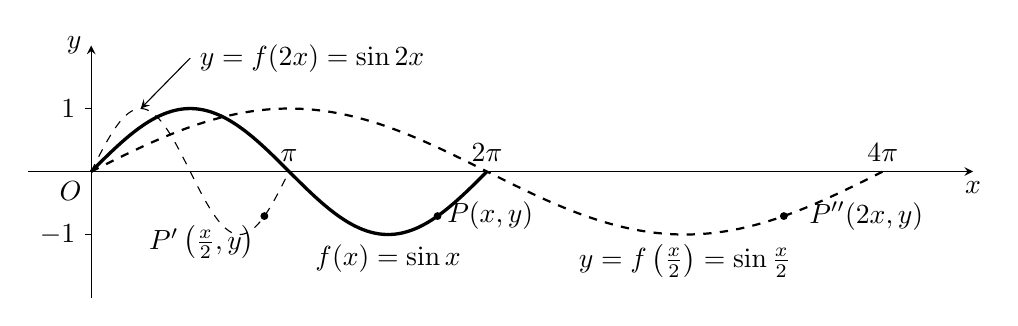
\begin{tikzpicture}[>=stealth, scale=.8]
    \draw[->](-1,0)--(14,0)node[below]{$x$};
\draw[->](0,-2)--(0,2)node[left]{$y$};
\node[below left]{$O$};
\draw[thick, dashed, domain=0:4*pi, smooth, samples=100]plot(\x, {sin(0.5*\x r)});
\draw[dashed, domain=0:pi, smooth, samples=100]plot(\x, {sin(2*\x r)});
\draw[very thick, domain=0:2*pi, smooth, samples=100]plot(\x, {sin(\x r)});
\foreach \x in {1,-1}
{
    \draw(0,\x)--(-.1,\x)node[left]{$\x$};
}
\node at (pi,0)[above]{$\pi$};
\node at (4*pi,0)[above]{$4\pi$};
\node at (2*pi,0)[above]{$2\pi$};
\node at (3*pi,-1)[below]{$y=f\left(\frac{x}{2}\right)=\sin \frac{x}{2}$};
\node at (3*pi/2,-1)[below]{$f(x)=\sin x$};
\draw[<-](pi/4,1)--(pi/2,1.8)node[right]{$y=f(2x)=\sin 2x$};


\draw[fill](2*pi-pi/4, -1.414/2)node[ right]{$P(x,y)$} circle (1.5pt);
\draw[fill](4*pi-pi/2, -1.414/2)node[ right=.2cm]{$P''(2x,y)$} circle (1.5pt);
\draw[fill](pi-pi/8, -1.414/2)node[below left]{$P'\left(\frac{x}{2},y\right)$} circle (1.5pt);


\end{tikzpicture}
    \caption{}
\end{figure}

\subsection{$y=|f(x)|$}
欲作$y=|f(x)|$的图象,只须把(*)的图象上纵坐标$y$为负值的点作出关于$x$轴的对称点(图3.24),即使(*)上的每个点$(x,y)\to (x,|y|)$.
\begin{figure}[htp]
    \centering
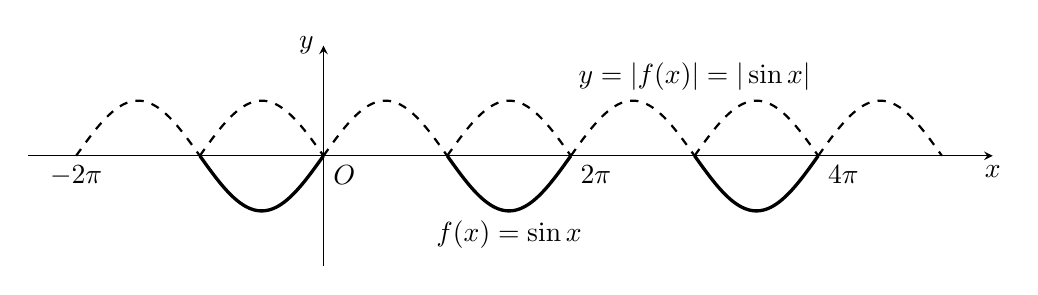
\begin{tikzpicture}[>=stealth, xscale=.5, yscale=.7]
    \draw[->](-7.5,0)--(17,0)node[below]{$x$};
\draw[->](0,-2)--(0,2)node[left]{$y$};
\node[below right]{$O$};
\foreach \y in {-1,0,1}
{
    \draw[very thick, domain=pi:2*pi, smooth, samples=100]plot(\x+\y*2*pi, {sin(\x r)});
}
\foreach \y in {-2,-1,0,...,4}
{
    \draw[thick, dashed, domain=0:pi, smooth, samples=100]plot(\x+\y*pi, {sin(\x r)});
}

\node at (-2*pi,0)[below]{$-2\pi$};
\node at (4*pi,0)[below right]{$4\pi$};
\node at (2*pi,0)[below right]{$2\pi$};

\node at (3*pi/2,-1)[below]{$f(x)=\sin x$};
\node at (3*pi,1)[above]{$y=|f(x)|=|\sin x|$};


\end{tikzpicture}
    \caption{}
\end{figure}

\subsection{$y=f(|x|)$}

很明显,$y=f(|x|)$是个偶函数,其图象关于$y$轴对称. 其次,由于 
\[f(|x|)=\begin{cases}
    f(x),& x\ge 0\\
    f(-x),& x<0
\end{cases}\]
可见,$y=f(|x|)$在$x\ge 0$的区间上图象与(*)完全相同。由此,欲作$y=f(|x|)$的图象,可以分两步:第一步,$x\ge 0$部分同(*);第二步,把(*)上$x>0$部分作关于$y$轴的对称图形就可得到$x<0$部分的图象(图3.25).

\begin{figure}[htp]
    \centering
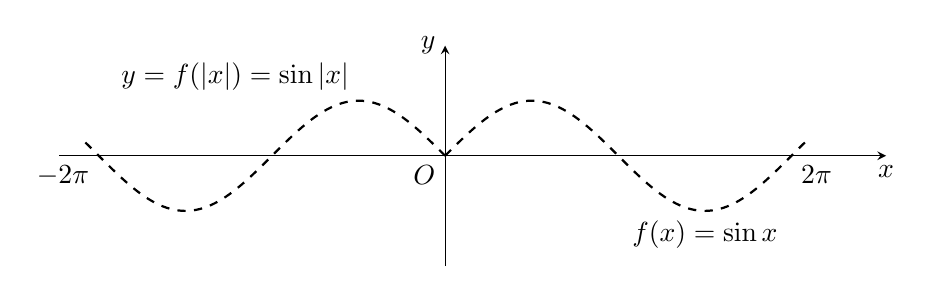
\begin{tikzpicture}[>=stealth, scale=.7]
    \draw[->](-7,0)--(8,0)node[below]{$x$};
\draw[->](0,-2)--(0,2)node[left]{$y$};
\draw[thick, dashed, domain=0:2*pi+.3, smooth, samples=100]plot(\x, {sin(\x r)});
\draw[thick, dashed, domain=0:2*pi+.3, smooth, samples=100]plot(-\x, {sin(\x r)});

\node at (-2*pi,0)[below left]{$-2\pi$};
\node at (2*pi,0)[below right]{$2\pi$};
\node[below left]{$O$};
\node at (3*pi/2,-1)[below]{$f(x)=\sin x$};
\node at (-pi/2,1)[above left]{$y=f(|x|)=\sin |x|$};


\end{tikzpicture}
    \caption{}
\end{figure}

\subsection{$y=\frac{1}{f(x)}$}

欲作$y=\frac{1}{f(x)}$的图象,只须把(*)的图象上的每一个点$(x,
y)\to \left(x,\; \frac{1}{y}\right)$(图3.26).

\begin{figure}[htp]
    \centering
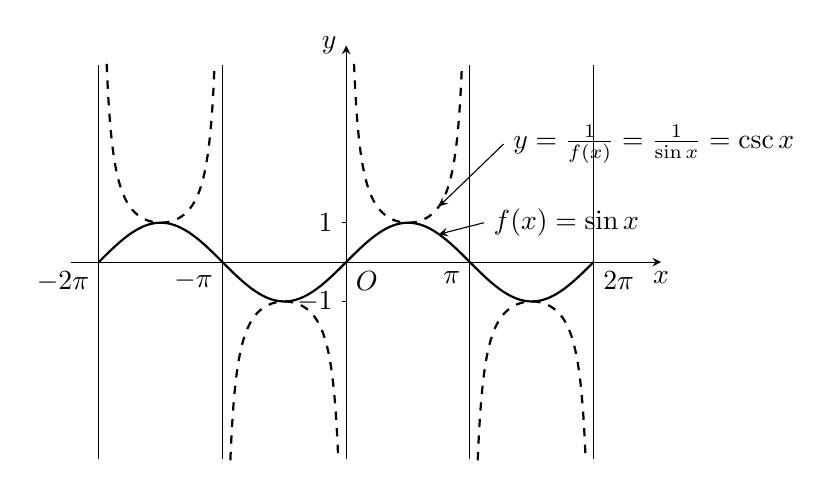
\begin{tikzpicture}[>=stealth, scale=.5]
    \draw[->](-7,0)--(8,0)node[below]{$x$};
\draw[->](0,-5)--(0,5.5)node[left]{$y$};
\draw[thick, domain=-2*pi:2*pi, smooth, samples=100]plot(\x, {sin(\x r)});
\draw(0,1)--(-.1,1)node[left]{$1$};
\draw(0,-1)--(-.1,-1)node[left]{$-1$};

\node at (-2*pi,0)[below left]{$-2\pi$};
\node at (pi,0)[below left]{$\pi$};
\node at (-pi,0)[below left]{$-\pi$};
\node at (2*pi,0)[below right]{$2\pi$};
\node[below right]{$O$};

\foreach \x in {-2,-1,1,2}
{
    \draw(\x*pi,5)--(\x*pi,-5);
}
\draw[thick, dashed, domain=0+.2:pi-.2, smooth, samples=100]plot(\x, {1/sin(\x r)});
\draw[thick, dashed, domain=0+.2:pi-.2, smooth, samples=100]plot(\x-2*pi, {1/sin(\x r)});
\draw[thick, dashed, domain=0+.2:pi-.2, smooth, samples=100]plot(\x+pi, {-1/sin(\x r)});
\draw[thick, dashed, domain=0+.2:pi-.2, smooth, samples=100]plot(\x-pi, {-1/sin(\x r)});

\draw[<-](3*pi/4, 1.414/2)--(3.5,1)node[right]{$f(x)=\sin x$};
\draw[<-](3*pi/4, 2/1.414)--(4,3)node[right]{$y=\frac{1}{f(x)}=\frac{1}{\sin x}=\csc x$};
\end{tikzpicture}
    \caption{}
\end{figure}

以上,讲了九种图象的几何变换,它们对今后的学习都很重要。应弄清原理,掌握作法。


\begin{example}
    用几何变换的方法作函数$y=\sin(-x)$的图象。
\end{example}

\begin{solution}
    \textbf{方法1:} 作$y=\sin x$关于$y$轴的对称曲线就是$y=\sin(-x)$的图象(图3.27).
\begin{figure}[htp]
    \centering
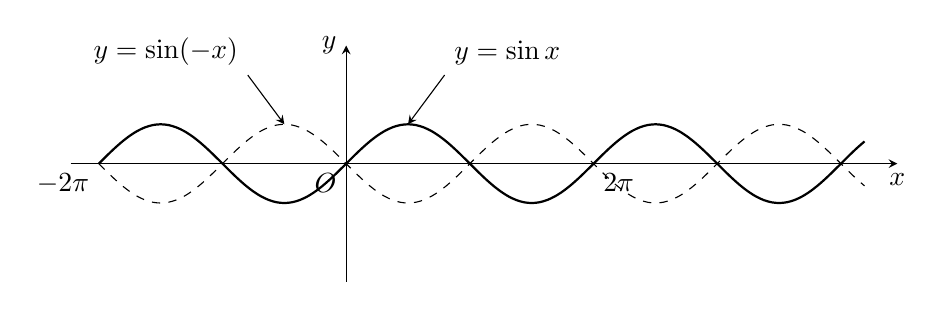
\begin{tikzpicture}[>=stealth, scale=.5]
    \draw[->](-7,0)--(14,0)node[below]{$x$};
\draw[->](0,-3)--(0,3)node[left]{$y$};
\draw[thick, domain=-2*pi:4*pi+.6, smooth, samples=100]plot(\x, {sin(\x r)});
\draw[dashed, domain=-2*pi:4*pi+.6, smooth, samples=100]plot(\x, {-sin(\x r)});
\node at (-2*pi,0)[below left]{$-2\pi$};

\node at (2*pi,0)[below right]{$2\pi$};
\node[below left]{$O$};

\draw[<-](pi/2, 1)--(2.5,2.25)node[above right]{$y=\sin x$};
\draw[<-](-pi/2, 1)--(-2.5,2.25)node[above left]{$y=\sin (-x)$};


\end{tikzpicture}
    \caption{}
\end{figure}
\end{solution}

\begin{thm}
    {思考题} 对此例,你还能想到别的变换方法吗?
\end{thm}

\begin{example}
    用几何变换的方法,由$y=\sin x$的图象作$y=\sin\frac{x}{2}$的图象。
\end{example}


\begin{solution}
    根据$y=\sin x$的图象,作横向伸缩变换$(x,y)\to \left(\frac{x}{\frac{1}{2}},\; y\right)$
,即$(2x,y)$(图3.28).
\begin{figure}[htp]
    \centering
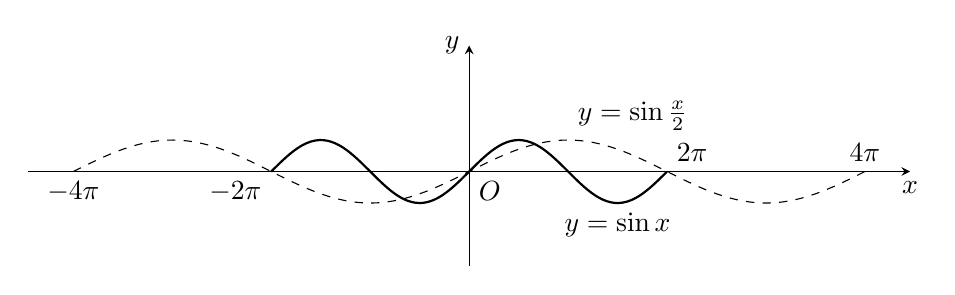
\begin{tikzpicture}[>=stealth, scale=.4]
    \draw[->](-14,0)--(14,0)node[below]{$x$};
\draw[->](0,-3)--(0,4)node[left]{$y$};
\draw[thick, domain=-2*pi:2*pi, smooth, samples=100]plot(\x, {sin(\x r)});
\draw[dashed, domain=-2*pi:2*pi, smooth, samples=100]plot(2*\x, {sin(\x r)});
\node at (-2*pi,0)[below left]{$-2\pi$};
\node at (-4*pi,0)[below ]{$-4\pi$};

\node at (2*pi,0)[above right]{$2\pi$};
\node at (4*pi,0)[above ]{$4\pi$};
\node[below right]{$O$};

\node at (1.5*pi,-1)[below]{$y=\sin x$};
\node at (pi,1)[above right]{$y=\sin\frac{x}{2}$};


\end{tikzpicture}
    \caption{}
\end{figure}
    \end{solution}

\begin{example}
    函数$y=3\sin\left(2x+\frac{\pi}{3}\right)$
的图象,可看作$y=\sin x$
的图象经过哪些几何变换得到的?
\end{example}

\begin{analyze}
既有纵向和横向的压缩变换,又有横向平移。还有一个变换的顺序问题。
\end{analyze}

\begin{solution}
    \textbf{解法1:}(先压后移,见图3.29)


    我们先把$y=3\sin\left(2x+\frac{\pi}{3}\right)$写成$y=3\sin2\left(x+\frac{\pi}{6}\right)$, 
    则
\[\begin{split}
    y=\sin x & \xrightarrow[(x,y)\to (x,3y)]{\text{纵压}} y=3\sin x \xrightarrow[(x,y)\to \left(\tfrac{x}{2},y\right)]{\text{横压} }y=3\sin 2x\\
&\xrightarrow[(x,y)\to \left(x-\tfrac{\pi}{6},y\right)]{\text{左移}\tfrac{\pi}{6}} y=3\sin 2\left(x+\frac{\pi}{6}\right)
\end{split}\]    
    
\begin{figure}[htp]
    \centering
\begin{tikzpicture}[>=stealth]
    \draw[->](-1,0)--(7,0)node[below]{$x$};
\draw[->](0,-4)--(0,4)node[left]{$y$};
\draw[thick, domain=0:2*pi, smooth, samples=100]plot(\x, {sin(\x r)});
\draw[dashed, domain=0:2*pi, smooth, samples=100]plot(\x, {3*sin(\x r)});
\draw[thick, dashed, domain=0:2*pi, smooth, samples=100]plot(0.5*\x, {3*sin(\x r)});
\draw[very thick, dashed, domain=0:2*pi, smooth, samples=100]plot(0.5*\x-pi/6, {3*sin(\x r)});

\node at (2*pi,0)[above]{$2\pi$};
\node at (pi,0)[above]{$\pi$};
\node at (pi/2,0)[above right]{$\tfrac{\pi}{2}$};
\node at (-pi/6,0)[below]{$-\tfrac{\pi}{6}$};
\node at (5*pi/6,0)[below left]{$\tfrac{5\pi}{6}$};

\node[below right]{$O$};

\foreach \x in {1,2,3}
{
    \draw(0,\x)--(-.1,\x)node[left]{$\x$};
    \draw(0,-\x)node[right]{$-\x$}--(-.1,-\x);
}
\draw[<-](pi/12,3)--(1,3.5)node[right]{$y=3\sin2\left(x+\frac{\pi}{6}\right)$};
\draw[<-](pi/2,1)--(2.5,1.5)node[right]{$y=\sin x$};
\draw[<-](3*pi/4,-3)--(3,-3.5)node[right]{$y=3\sin 2x$};
\draw[<-](2*pi-pi/4, -1.414*3/2)--(6,-2.4)node[right]{$y=3\sin x$};


\end{tikzpicture}
    \caption{}
\end{figure}



    \textbf{解法2:}(先移后压,见图3.30):
\[\begin{split}
    y=\sin x & \xrightarrow[(x,y)\to \left(x-\tfrac{\pi}{3}, y\right)]{\text{左移}\tfrac{\pi}{3}} y=\sin \left(x+\frac{\pi}{3}\right) \xrightarrow[(x,y)\to \left(\tfrac{x}{2},y\right)]{\text{横压} }y=\sin \left(2x+\frac{\pi}{3}\right)\\
&\xrightarrow[(x,y)\to \left(x,3y\right)]{\text{纵压}} y=3\sin \left(2x+\frac{\pi}{3}\right)
\end{split}\]   

\begin{figure}[htp]
    \centering
\begin{tikzpicture}[>=stealth]
    \draw[->](-2,0)--(7,0)node[below]{$x$};
\draw[->](0,-4)--(0,4)node[left]{$y$};
\draw[thick, domain=0:2*pi, smooth, samples=100]plot(\x, {sin(\x r)});
\draw[dashed, domain=0:2*pi, smooth, samples=100]plot(\x-pi/3, {sin(\x r)});
\draw[thick, dashed, domain=0:2*pi, smooth, samples=100]plot(0.5*\x-pi/6, {sin(\x r)});
\draw[very thick, dashed, domain=0:2*pi, smooth, samples=100]plot(0.5*\x-pi/6, {3*sin(\x r)});

\node at (2*pi,0)[above]{$2\pi$};
\node at (pi,0)[above]{$\pi$};
\node at (5*pi/3,0)[above]{$\tfrac{5\pi}{3}$};
% \node at (pi/2,0)[above right]{$\tfrac{\pi}{2}$};
\node at (-pi/6,0)[below]{$-\tfrac{\pi}{6}$};
\node at (-pi/3,0)[below]{$-\tfrac{\pi}{3}$};
% \node at (5*pi/6,0)[below left]{$\tfrac{5\pi}{6}$};

\node[below right]{$O$};

\foreach \x in {1,2,3}
{
    \draw(0,\x)--(-.1,\x)node[left]{$\x$};
    \draw(0,-\x)node[right]{$-\x$}--(-.1,-\x);
}
\draw[<-](3*pi/4-pi/6,-3)--+(1,-.25)node[right]{$y=3\sin\left(2x+\frac{\pi}{3}\right)$};
\draw[<-](pi/2,1)--(2.5,1.5)node[right]{$y=\sin x$};
\draw[<-](3*pi/4-pi/6,-1)--+(.75,-1.25)node[right]{$y=\sin\left(2x+\frac{\pi}{3}\right) $};
\draw[<-](3*pi/2-pi/3, -1)--+(1,-.5)node[right]{$y=\sin \left(x+\frac{\pi}{3}\right)$};


\end{tikzpicture}
    \caption{}
\end{figure}
\end{solution}

\begin{remark}
对于函数$y=A\sin(\omega x+\varphi)$的作图上面讲了两种方法:一是描点法(特别是用“五点法”作简图),二是几何图形的变换法。在实际作简图时,主要用五点法。讲几何变换法主要是弄清简单函数与复合函数图象之间的联系,为今后的研究提供方便。
\end{remark}    

在物理学中,我们常常用函数
\begin{equation}
    y=A\sin(\omega x+\varphi),\qquad A>0,\; \omega>0,\; x\in[0,+\infty) \tag{1}
\end{equation}
表示一个振动量(如交流电的电流强度或电压;弹性体振动时,质点离开平衡位置的距离;…… 因此,(1)又称为\textbf{振动函数}. (要特别注意:对振动函数而言,条件$A>0,\; \omega>0,\; x\in[0,+\infty)$是非常必要的。它们都有明显的物理意义)。此时,$A$表示振动量离开平衡位置的最大距离,通常称为这个振动的\textbf{振幅};往复振动一次所需的时间$T=\frac{2\pi}{\omega}$,叫做振动的\textbf{周期};单位时间内往复振动的次数$f=\frac{1}{T}=\frac{\omega}{2\pi}$,叫做振动的\textbf{频率};$\omega x+\varphi$叫做\textbf{相位},$\varphi$叫做\textbf{初相}(即为$x=0$时的相位).


\begin{example}
当$y=2\sin\left(-2x+\frac{\pi}{3}\right)$描写振动时,求它的振幅、周期、频率、相位和初相。
\end{example}

\begin{analyze}
    这里,$x$的系数小于零,不合振动函数的要求. 因此,先要把函数式变形。
\end{analyze}

\begin{solution}
利用$\sin x=\sin(\pi-x)$, 得
\[y=2\sin\left(-2x+\frac{\pi}{3}\right)=2\sin\left(\pi+2x-\frac{\pi}{3}\right)=2\sin\left(2x+\frac{2\pi}{3}\right)\]

$\therefore\quad 
A=2,\quad T=\frac{2\pi}{\omega}=\frac{2\pi}{2}=\pi,\quad f=\frac{1}{T}=\frac{1}{\pi}$,相位是$2x+\frac{2\pi}{3}$,初相是$\frac{2\pi}{3}$.
\end{solution}



\begin{example}
    当$y=-3\sin\left(4x+\frac{\pi}{6}\right)$描写振动时,求其振幅、周期、频率、相位和初相。
\end{example}

\begin{analyze}
这里,正弦函数的系数小于零,不合振动函数的要求,需要把函数式先变形.
\end{analyze}

\begin{solution}
    利用$-\sin x=\sin(-x)$, 得
\[\begin{split}
    y&=-3\sin\left(4x+\frac{\pi}{6}\right)=3\sin\left(-4x-\frac{\pi}{6}\right)\\
    &=3\sin\left(\pi+4x+\frac{\pi}{6}\right)=3\sin\left(4x+\frac{7\pi}{6}\right)
\end{split}\]

$\therefore\quad A=3,\quad T=\frac{2\pi}{\omega}=\frac{2\pi}{4}=\frac{\pi}{2},\quad f=\frac{1}{T}=\frac{2}{\pi}$,相
位是$4x+\frac{7\pi}{6}$,初相是$\frac{7\pi}{6}$.
\end{solution}

\section*{习题六}
\begin{center}
    \bfseries A
\end{center}

\begin{enumerate}
    \item 下列函数的图象,可看作由$y=x^2$的图象经过哪些几何变换得来的(不必画图):
\begin{multicols}{2}
\begin{enumerate}[(1)]
    \item $y=3(x-2)^2+1$
    \item $y=-2x^2-12x-20$
\end{enumerate}    
\end{multicols}

    
    \item  下列函数的图象,可看作由$y=\sin x$的图象经过哪些几何变换得来的(不必画图)?同时说出每个函数的周期:
\begin{multicols}{2}
\begin{enumerate}[(1)]
    \item $y=\sin \frac{3}{2}x$
    \item $y=-3\sin x$
    \item $y=\sin\left(x+\frac{\pi}{4}\right)$
    \item $y=2\sin\left(3x+\frac{\pi}{3}\right)$
\end{enumerate}    
\end{multicols}

    \item 下列函数的图象,可看作由$y=\cos x$的图象经过哪些几何变换得来的(不必画图)?同时说出每个函数的周期:
\begin{multicols}{2}
\begin{enumerate}[(1)]
\item $y=-\cos x +2$
\item $y=2\cos4x$
\item $y=\cos\left(x-\frac{\pi}{3}\right)$
\item $y=2-3\cos\left(2x-\frac{\pi}{4}\right)$
\end{enumerate}
\end{multicols}

\item 当下列函数描写振动时,写出它的振幅、周期、频率、相位和初相(“写出”题,不必有过程):
\begin{multicols}{2}
\begin{enumerate}[(1)]
    \item $y=2\sin\left(5x+\frac{\pi}{3}\right)$
    \item $y=3\cos\left(2x+\frac{\pi}{3}\right)$
\end{enumerate}
\end{multicols}
\item \begin{enumerate}[(1)]
\item $y=|\sin x|$的最小正周期是\blank;
\item $y=2\left|\sin\left(4x-\frac{\pi}{3}\right)\right|$的最小正周期是\blank.
\end{enumerate}

\item 电流强度$I$随时间$t$变化的函数关系是$I=A\sin\omega t$. 设$\omega=100\pi$(弧度/秒),$A=5$(安培),
\begin{enumerate}[(1)]
\item 求电流强度$I$变化的周期与频率;
\item 当$t=0,\; \frac{1}{100},\; \frac{1}{50}$(秒)时,求相应的$I$;
\item 画出$I$随$t$变化的图象(以0.5cm表示1安培;以1cm表示$\frac{1}{100}$秒)。
\end{enumerate}
\end{enumerate}

\begin{center}
    \bfseries B
\end{center}
\begin{enumerate}\setcounter{enumi}{6}
    \item 当下列函数描写振动时,求出它的振幅、周期、频率、相位和初相:
\begin{multicols}{2}
\begin{enumerate}[(1)]
    \item $y=6\sin\left(-3x+\frac{\pi}{4}\right)$
    \item $y=-2\sin\left(4x-\frac{\pi}{5}\right)$
\end{enumerate}
\end{multicols}

\item 弹簧挂着的小球作上下振动,它在$t$秒钟时相对于平衡位置(就是静止时的位置)的高度$h$厘米由下列关系决定。
\[h=2\sin\left(t+\frac{\pi}{4}\right)\]
以$t$为横坐标,$h$为纵坐标,作出这个函数在一个周期内的图象,并回答下列问题:
\begin{enumerate}[(1)]
\item 小球在开始振动时(即$t=0$时)的位置在哪里?
\item 小球的最高点和最低点与平衡位置的距离分别是多少?
\item 经过多少时间,小球往复振动一次(周期)?
\item 每秒钟小球能往复振动多少次(频率)?   
\end{enumerate}

\item 一根长$\ell$厘米的线,一端固定,另一端悬挂一个小球。小球摆动时,离开平衡位置的位移$S$(厘米)和时间$t$(秒)的函数关系是:
\[S=3\cos\left(\sqrt{\frac{g}{\ell}}t+\frac{\pi}{3}\right)\]
\begin{enumerate}[(1)]
\item 求小球摆动的周期;
\item 已知$g=$980厘米/秒$^2$,要使小球摆动的周期是1秒,线的长度$\ell$应当是多少厘米(精确到0.1厘米,$\pi$取3.14)?
\end{enumerate}
\end{enumerate}

\section{正切函数与余切函数的图象}
利用三角函数线作正切函数与余切函数的图象也是很容易的。

因为$y=\tan x,\; x\in\R$且$x\ne \frac{\pi}{2}+k\pi\; (k\in\Z)$的周期(最小正
周期)是$\pi$,因而,可以先画它的一个周期$x\in\left(-\frac{\pi}{2},\; \frac{\pi}{2}\right)$的图象(图3.31)。然后,根据正切函数的周期性,再把图象向左、右延展,得出$x\in\left(-\frac{\pi}{2}+k\pi,\; \frac{\pi}{2}+k\pi\right),\; k\in\Z$
上的图象(图3.32),它称为\textbf{正切曲线}. 可以看出,它是由相互平行且等距的直线隔开的\textbf{无穷多支}全同的曲线构成的。

\begin{figure}[htp]
    \centering
\begin{tikzpicture}[>=stealth, scale=1.3]
\draw[->](-1.5,0)--(5.5,0)node[below]{$x$};
\draw[->](3,-3)--(3,3)node[left]{$y$};
\node at (3,0)[below right]{$O$};
\node at (1,0)[below right]{$A$};
\node at (-pi/2+3,0)[above left]{$-\tfrac{\pi}{2}$};
\node at (pi/2+3,0)[below right]{$\tfrac{\pi}{2}$};


\draw(0,0) circle (1);
\draw(0,1)node[above]{$B$}--(0,-1)node[below]{$B'$};
\draw(1,-2.5)--(1,2.5);
\foreach \x in {1,2,-1,-2}
{
    \draw(3,\x)node[left]{$\x$}--(3.1,\x);
}
\foreach \x in {pi*.5, -pi*.5}
{
    \draw[dashed](\x+3,-3)--(\x+3,3);
}

\draw[domain=-pi/2+.32:pi/2-.32, smooth, very thick, samples=100]plot(\x+3, {tan(\x r)});

\draw(0,0)--(1,1.732)--(pi/3+3,1.732)--(pi/3+3,0)node[below]{$\tfrac{\pi}{3}$};
\draw(0,0)--(1,-1.732)--(-pi/3+3,-1.732)--(-pi/3+3,0)node[above]{$-\tfrac{\pi}{3}$};
\draw(0,0)--(1,0.58)--(pi/6+3,0.58)--(pi/6+3,0)node[below]{$\tfrac{\pi}{6}$};
\draw(0,0)--(1,-0.58)--(-pi/6+3,-0.58)--(-pi/6+3,0)node[above]{$-\tfrac{\pi}{6}$};

\node at (1.5,-3)[below right]{$y=\tan x\quad x\in\left(-\frac{\pi}{2},\; \frac{\pi}{2}\right)$};
\end{tikzpicture}
    \caption{}
\end{figure}

正切曲线体现了前面研究过的\textbf{正切函数的性质}:
\begin{enumerate}[(1)]
\item 定义域为$x\in\R$,且$x\ne \frac{\pi}{2}+k\pi\; (k\in\Z)$[结合图3.32,应该理解:函数$y=\tan x$在$x= \frac{\pi}{2}+k\pi\; (k\in\Z)$上无定义];
\item 值域为$(-\infty,+\infty)$[从图上看得很清楚:在区间$\left(-\frac{\pi}{2}+k\pi,\; \frac{\pi}{2}+k\pi\right)\; (k\in\Z)$ 的两个端点内侧,当$x$无限地接近$\frac{\pi}{2}+k\pi\; (k\in\Z)$时,函数值可以大过任何正数,我们把这种情况记为$\tan x\to +\infty$(读作趋向正无穷大);当$x$无限地接近$-\frac{\pi}{2}+k\pi\; (k\in\Z)$时,函数值和上述情况恰好相反,记为$\tan x\to -\infty$(读作趋向负无穷大)。这就是说,$x$可以取任意实数值,但没有最大值和最小值,因此值域是$(-\infty,+\infty)$,或说成值域为$\R$];
\item 周期性:是定义域上的周期函数,周期为$\pi$;
\item 增减性:$\tan x$在每个开区间$\left(-\frac{\pi}{2}+k\pi,\; \frac{\pi}{2}+k\pi\right)\; (k\in\Z)$内都是增函数(但不能说,在它的整个定义域上是增函数,这一点从图3.32看得很清楚);
\item 奇偶性:由于任取$x\in D$,都有$\tan (-x)=-\tan x$, 知道$y=\tan x$是奇函数(从图象上也看得很清楚,图象关于原点对称)。
\end{enumerate}

\begin{figure}[htp]
    \centering
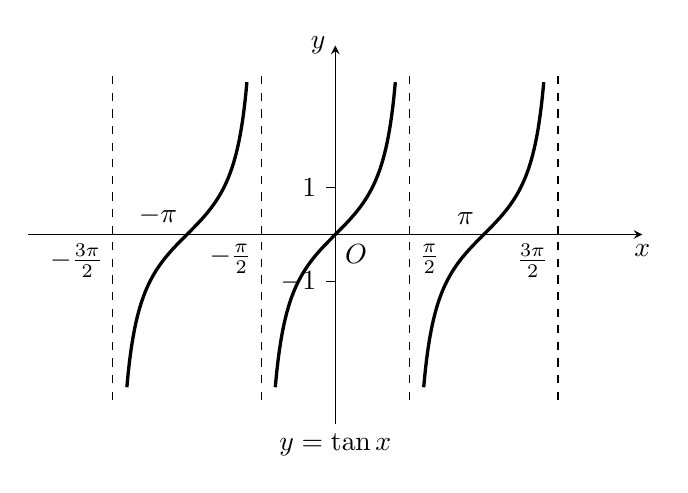
\begin{tikzpicture}[>=stealth, scale=.6]
    \draw[->](-6.5,0)--(6.5,0)node[below]{$x$};
    \draw[->](0,-4)node[below]{$y=\tan x$}--(0,4)node[left]{$y$};
    \node at (0,0)[below right]{$O$};    
    \draw[domain=-pi/2+.3:pi/2-.3, smooth, very thick, samples=100]plot(\x, {tan(\x r)});
    \draw[domain=-pi/2+.3:pi/2-.3, smooth, very thick, samples=100]plot(\x-pi, {tan(\x r)});
    \draw[domain=-pi/2+.3:pi/2-.3, smooth, very thick, samples=100]plot(\x+pi, {tan(\x r)});
\foreach \x in {-1.5,-.5,1.5,.5}
{
    \draw[dashed](\x*pi,-3.5)--(\x*pi,3.5);
}

\node at (-pi,0)[above left]{$-\pi$};
\node at (pi,0)[above left]{$\pi$};
\node at (-pi/2,0)[below left]{$-\frac{\pi}{2}$};
\node at (-pi*1.5,0)[below left]{$-\frac{3\pi}{2}$};
\node at (pi*1.5,0)[below left]{$\frac{3\pi}{2}$};
\node at (pi/2,0)[below right]{$\frac{\pi}{2}$};

\foreach \x in {1,-1}
{
    \draw(0,\x)--(-.2,\x)node[left]{$\x$};
}

\end{tikzpicture}
    \caption{}
\end{figure}

与作余弦曲线相类似的方法,可以作出余切函数$y=\cot x,\; x\in\R$,且$x\ne k\pi \; (k\in\Z)$的图象(图3.33),称为\textbf{余切曲线},它体现了\textbf{余切函数的性质}:
\begin{enumerate}[(1)]
    \item 定义域为$x\in\R$,且$x\ne k\pi\; (k\in\Z)$;
    \item 值域为$(-\infty,+\infty)$;
    \item 周期性:是定义域上的周期函数,周期为$\pi$;
    \item 增减性:$\cot x$在每个开区间$(0+k\pi,\; \pi+k\pi),\; k\in\Z$内,都是减函数(但不能说,是整个定义域上的减函数);
    \item 奇偶性:$\cot x$是奇函数。
\end{enumerate}


\begin{figure}[htp]
    \centering
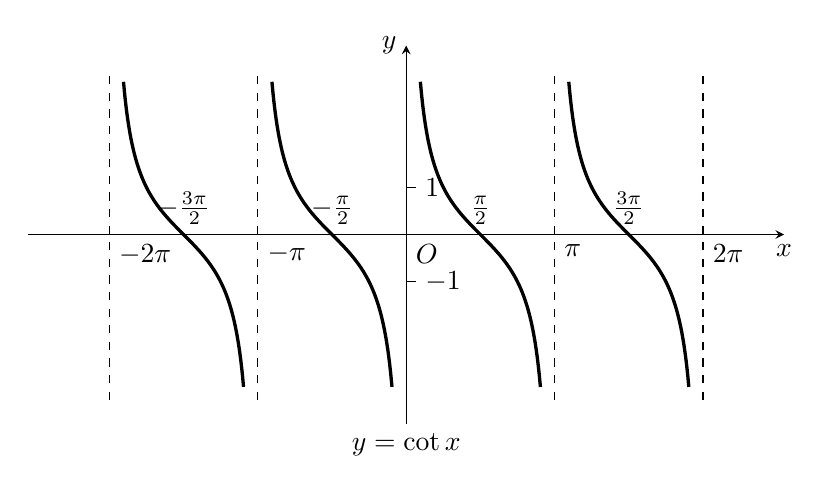
\begin{tikzpicture}[>=stealth, scale=.6]
    \draw[->](-8,0)--(8,0)node[below]{$x$};
    \draw[->](0,-4)node[below]{$y=\cot x$}--(0,4)node[left]{$y$};
    \node at (0,0)[below right]{$O$};    
    \draw[domain=.3:pi-.3, smooth, very thick, samples=100]plot(\x, {1/tan(\x r)});
    \draw[domain=.3:pi-.3, smooth, very thick, samples=100]plot(\x+pi, {1/tan(\x r)});
    \draw[domain=.3:pi-.3, smooth, very thick, samples=100]plot(\x-pi, {1/tan(\x r)});
    \draw[domain=.3:pi-.3, smooth, very thick, samples=100]plot(\x-2*pi, {1/tan(\x r)});

\foreach \x in {1,2,-1,-2}
{
    \draw[dashed](\x*pi,-3.5)--(\x*pi,3.5);
}
\node at (pi,0)[below right]{$\pi$};
\node at (-pi,0)[below right]{$-\pi$};
\node at (2*pi,0)[below right]{$2\pi$};
\node at (-2*pi,0)[below right]{$-2\pi$};

\node at (-pi/2,0)[above]{$-\frac{\pi}{2}$};
\node at (pi/2,0)[above]{$\frac{\pi}{2}$};
\node at (-pi*1.5,0)[above]{$-\frac{3\pi}{2}$};
\node at (pi*1.5,0)[above]{$\frac{3\pi}{2}$};


\foreach \x in {1,-1}
{
    \draw(0,\x)--(.2,\x)node[right]{$\x$};
}

\end{tikzpicture}
    \caption{}
\end{figure}

\begin{example}
求函数$y=\cot\left(3x-\frac\pi4\right)$的定义域、周期和单调区间。
\end{example}


\begin{solution}
    欲使$y=\cot\left(3x-\frac{\pi}{4}\right)$有意义,须
    $x\in \R$, 且$3x-\frac\pi4\neq k\pi\; \left(k\in \Z\right)$, 即
\[  x\in \R,\; \text{且}\;  x\neq \frac{k\pi}{3}+ \frac {\pi} {12}\quad ( k\in \Z)\]    

$\therefore\quad $函数 的定义 域为$\left\{x\Big| x\in\R,\; \text{且}\;  x\neq \frac {k\pi}{3}+ \frac \pi {12},\quad  k\in \Z \right\}$

设常数$T>0$, 则$f(x)=\cot \left(3x-\frac\pi4\right)$,
$$f(x+T)=\cot \left(3x-\frac{\pi}{4}+3T\right)$$

欲使$T$为$f(x)$的周期,须任取$x\in D$, 都有
$$\cot\left(3x-\frac{\pi}{4}\right)=\cot\left(3x-\frac{\pi}{4}+3T\right)$$
利用$y=\cot x$的周期为$\pi$, 得$3T=\pi\; \left(k\in \Z\right)\Rightarrow T=\frac{\pi}{3}\; (k\in \Z)$,

$\therefore\quad  T_{\text{最小正}}=\frac{\pi}{3}$.

当$0+k\pi<3x-\frac{\pi}{4}<\pi+k\pi\; (k\in \Z)$时函数为减函数
即
$$\frac\pi{12}+\frac{k\pi}3<x<\frac{5\pi}{12}+\frac{k\pi}3 \quad \left(k\in \Z\right)$$

$\therefore\quad $ 单调减区间为$\left ( \frac \pi {12}+ \frac {k\pi }3,\; \frac {5\pi }{12}+ \frac {k\pi }3\right ),\quad k\in \Z$, 没有单调增区间。
\end{solution}



\begin{example}
求$f(x)=\tan x-\cot x$的定义域、周期、值域。

\end{example}

\begin{solution}
要使$f(x)$有意义,须$\tan x$, $\cot x$都有意义,

$\therefore\quad $ 定义域为$\left\{x\Big| x\in \R,\; \text{且 }\; x\neq\frac\pi2 \cdot k,\:k\in \Z\right\}$

欲求$f(x)$的周期、值域,应将$f(x)$化成一个三角函数.
\[\begin{split}
    f(x)&=\frac{\sin x}{\cos x}-\frac{\cos x}{\sin x}=\frac{\sin^2 x-\cos^2 x}{\sin x\cos x}\\ 
    &=-2\cdot \frac{\cos 2x}{\sin 2x}=-2\cot 2x
\end{split}\]
$\therefore\quad T=\frac{\pi}{2}$,值域为$\R$.
\end{solution}

\section*{习题七}
\begin{center}
    \bfseries A
\end{center}
\begin{enumerate}
    \item 求下列函数的定义域与值域
\begin{multicols}{2}
\begin{enumerate}[(1)]
    \item  $y= \cot\left ( 2x- \frac \pi 3\right )$
    \item $y= \tan x+ \cot x$
    \item $y= \frac 1{\tan x- \cot x}$
    \item $y= \frac 1{1+ \cot x}$
\end{enumerate}
\end{multicols}
    \item 写出下列函数的周期:
\begin{multicols}{2}
\begin{enumerate}[(1)]
    \item $y=\tan 3x$
    \item $y=\cot \frac{\pi}{2}$
    \item $y=\tan\left(x+\frac{\pi}{4}\right)$
    \item $y=\cot\left(2x-\frac{\pi}{4}\right)$
\end{enumerate}
\end{multicols}
  
    \item 下列函数中,哪些是奇函数?偶函数?非奇又非偶函数?
\begin{multicols}{2}
\begin{enumerate}[(1)]
    \item $y=2\tan 4x$
    \item $y= 1+\cot x$ 
    \item $y=-\tan x$
    \item $y= - |\cot x|$
\end{enumerate}
\end{multicols}
    \item 比较下列各组数中的大小,并说明理由。
\begin{multicols}{2}
\begin{enumerate}[(1)]
    \item $\tan \left(-\frac\pi5\right)$与$\tan\left(\frac{4\pi}{7}\right)$
    \item $\tan \frac{7\pi}8$与$\tan\frac\pi{16}$
\end{enumerate}\end{multicols}
\end{enumerate}

\begin{center}
    \bfseries B
\end{center}
\begin{enumerate}\setcounter{enumi}{4}
    \item 函数$y=\sqrt{\tan x-1}$的定义域是\blank,值域是\blank.
   
    \item   函数$y=\frac{\sqrt{x(6-x)}}{\tan x-\cot x}$ 的定义域是\blank.
    \item   设$\alpha,\beta\in \left(\frac{\pi}{2},\pi\right)$,且$\tan\alpha<\cot\beta$,那么必有(\qquad )
\begin{multicols}{2}
\begin{enumerate}[(A)]
    \item $\alpha<\beta$
    \item $\alpha>\beta$
    \item $\alpha+\beta<\frac{3\pi}{2}$
    \item $\alpha+\beta>\frac{3\pi}{2}$
\end{enumerate}
\end{multicols}
\end{enumerate}


\section{本章小结}

\subsection{知识结构分析}
本章以三角函数的定义和三角函数线为依据,全面研究了四个三角函数的性质和图象。

三角函数的图象如图3.34,结合图象可以进一步认识三角函数的性质.

\subsection{几点说明}
\begin{enumerate}
    \item 定义域是自变量$x$的取值范围,应特别注意$\tan x$, $\cot x$的无定义的点(间断点)。
    \item 值域是函数值的取值范围。弦函数的值域是$[-1,1]$.应该理解:$-1$是它们的最小值,1是它们的最大值,函数能取到$[-1,1]$中的任何值。切函数的值域是$(-\infty,+\infty)$,因而,它们无最小值也无最大值,它们能取到任何实数值。
    \item 表中列出的周期,指的都是最小正周期。今后无需说明,求函数的周期都是求最小正周期(如果最小正周期存在的话)。若要判断某函数是否是周期函数,根本的是使用定义.
    
    要结合三角函数,正确理解“周期函数”的定义和本质.会用“周期”的概念简化函数性质的研究。
    \item 函数的奇偶性,是其定义域上的整体性质,这一点必须清楚[如$y=\cos x\; (x\ge 0)$就不是偶函数]。当然,判断一个函数是否是奇(偶)函数,最根本的是使用奇(偶)函数的定义.
    \item 函数的单调性,是对其定义域上的子区间而言的。应特别注意,虽然在$\left(-\frac{\pi}{2}+2k\pi,\; \frac{\pi}{2}+2k\pi\right)$或$\left(\frac{\pi}{2}+2k\pi,\; \frac{3\pi}{2}+2k\pi\right)$,其中$k\in\Z$上$\tan x$都是增函数,但不能说它在其定义域是增函数。
    \item  对于函数$y=A\sin(\omega x+\varphi)$,其中$A\ne 0$,应会讨论它的各种性质,会用五点法画它的简图。知道它的图象可由$y=\sin x$的图象,经过怎样的几何变换得出来。
    \item 对于$\sin x$、 $\cos x$、 $\tan x$、$\cot x$,都要会用“五点法”画简图.
\end{enumerate}






\begin{example}
    
\end{example}

\begin{analyze}
    
\end{analyze}

\begin{solution}
    
\end{solution}



\begin{example}
    
\end{example}

\begin{analyze}
    
\end{analyze}

\begin{solution}
    
\end{solution}



\begin{example}
    
\end{example}

\begin{analyze}
    
\end{analyze}

\begin{solution}
    
\end{solution}



\begin{example}
    
\end{example}

\begin{analyze}
    
\end{analyze}

\begin{solution}
    
\end{solution}



\begin{example}
    
\end{example}

\begin{analyze}
    
\end{analyze}

\begin{solution}
    
\end{solution}


























